%************************************************
\chapter{Hot Dust}\label{ch:hotdust} 

% Refer to: 
% HotDustPaper/
 % summary-150309.ipynb
 % notes.md
 % correlations_summary_141204.ipynb
 % correlations_summary.md
 % various *.md 



%************************************************

While many authors have focused on studies of specific sub-sets of active galactic nuclei with extreme observational properties, what is missing is an understanding of how these extreme subsets relate to the population as a whole. 
I have made some progress in addressing this problem using multi-wavelength spectral energy distributions of large ($\sim$100,000) samples of quasars. 
I have constructed an SED model which is able to reproduce the average optical to near-infrared (NIR) colours of 10,000s of AGNs spanning a broad range in redshift/luminosity. 
The goal of this work is to relate the intrinsic spread in SED properties to physical properties of the AGN. 

First we will present model, show it can reproduce the average optical to near-infrared (NIR) colours of 10,000s of AGNs spanning a broad range in redshift/luminosity. 
Then focus on the diversity in near-infrared emission, and relation to physical properties of quasars. 

\section{Data}

In the next two sections I will describe how I have modelled the SED in the quasar rest-frame UV to near-IR spectral region. 
We begin by fitting the same model to a large sample of quasars to emphasise common features, and then look for differences from the typical model in various sub-populations. 
The systematic study of the dependence of the SED shape on physical parameters has, until very recently, been limited by the difficulty in obtaining a large sample of quasars with good multi-wavelength coverage and large dynamic range in luminosity and redshift. 
In this work, we take advantage of a number of recent, sensitive, wide-field surveys, covering the UV to mid-IR spectral region. 
We will now describe these surveys, and how we combined them to create a large sample of quasars with multi-wavelength photometry.        

\section{Surveys}

\subsection{The Sloan Digital Sky Survey}

We use the spectroscopic quasar catalogues of the Sloan Digital Sky Survey \citep[SDSS;][]{york00} Seventh Data Release \citep[DR7Q;][]{schneider10} and Tenth Data Release \citep[DR10Q;][]{paris14}. 
The SDSS obtained images in five broad optical passbands: $u$ ($\lambda_{\rm eff} = 3543$\AA), $g$ ($\lambda_{\rm eff} = 4770$\AA), $r$ ($\lambda_{\rm eff} = 6231$\AA), $i$ ($\lambda_{\rm eff} = 7625$\AA), and $z$ ($\lambda_{\rm eff} = 9134$\AA). 
The SDSS spectra cover $\sim 3000 - 9000$\AA~ at a spectral resolution of $\sim 2000$. 

We use BEST point-spread function (PSF) magnitudes from the DR7Q catalogue, which are uncorrected for Galactic extinction. 
The Galactic extinction, which is calculated using the maps of \citet{schlegel98}, is given in the $u$ band only. The Galactic extinction in the $griz$ passbands is calculated using a Milky Way (MW) extinction curve \citep{pei92} and assuming an extinction to reddening ratio ${\rm A}(V) / {\rm E}(B-V) = 3.1$. 
We use the PSF magnitudes from the DR10Q catalogue, correcting for Galactic extinction using the maps of \citet{schlafly11}. 

SDSS uses `asinh' magnitudes, rather than conventional Pogson magnitudes. 
Although the photometry is intended to be on the AB system \citet{oke83}, the photometric zero-points are known to be slightly off the AB standard. 
To account for this we add 0.03 mag to the $u$, $g$, $r$ and $i$ magnitudes, and 0.05 mag to the $z$ magnitude.

DR7Q and DR10Q include 105,783 objects across 9380 deg$^2$, and 166,583 objects across 6,370 deg$^2$, respectively, with 16,420 objects in common to both catalogues. 
In Figure \ref{fig:histograms} we compare the distributions of redshift, apparent $i$ magnitude and absolute $i$ magnitude of objects in the two catalogues. 

\subsubsection{Redshift Distribution (Figure \ref{fig:histograms}; {\it Top panel})}

The median redshift of the DR7Q sample is 1.49 and 77\% are at redshifts $<$ 2. 
DR10Q quasars were selected to have redshifts $>2$ with the goal of studying the Ly-$\alpha$ forest; the smaller peaks in the distribution at $z \sim 0.8$ and $z \sim 1.6$ are due to degeneracies in the color selection space. At $z<2$ the incompleteness of the DR10Q catalogue is high, and so the DR7Q catalogue is more suitable for studying systematic changes in quasar properties with redshift. 

\subsubsection{Observed $i$ Magnitude Distribution (Figure \ref{fig:histograms}; {\it Middle panel})}

DR7Q quasar targets were primarily selected to have $i \leq 19.1$ if the colours were consistent with being at redshift $z < 3$, and $i \leq 20.2$ if consistent with $z > 3$ \citep{richards02}. 
The large number of objects at $z < 3$ with $i > 19.1$ were selected by algorithms other than the main quasar selection. 
For example, quasar targets were also selected if they matched within 2$''$ of an object in the Faint Images of the Radio Sky at Twenty-cm (FIRST) catalogue of radio sources \citep{becker95}. 
DR10Q targets were primarily selected to have g $\leq$ 22.0 or r $\leq$ 21.85, which means the DR10Q catalogue goes to much fainter magnitudes than the DR7Q catalogue and is, for example, more sensitive to populations of reddened quasars. 

\subsubsection{Absolute $i$ Magnitude Distribution (Figure \ref{fig:histograms}; {\it Middle panel})}

Both samples are composed primarily of luminous quasars; the absolute magnitude distributions are roughly symmetric around $M_i \simeq -26.0$ and $M_i \simeq -25.6$ for DR7Q and DR10Q respectively, with DR10Q extending to lower luminosities.  

\begin{figure}
  \centering
  \begin{minipage}[b]{0.5\textwidth}
    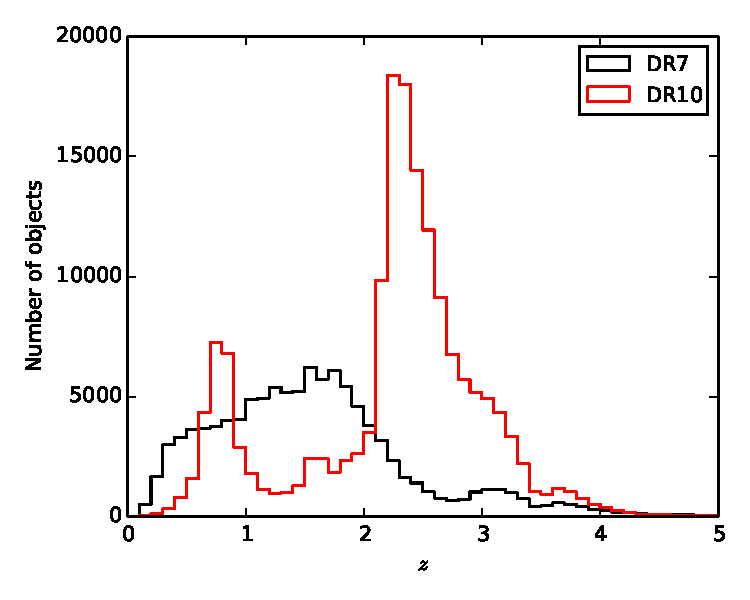
\includegraphics[width=\textwidth]{figures/chapter06/zhist}
  \end{minipage}\\
  \begin{minipage}[b]{0.5\textwidth}
    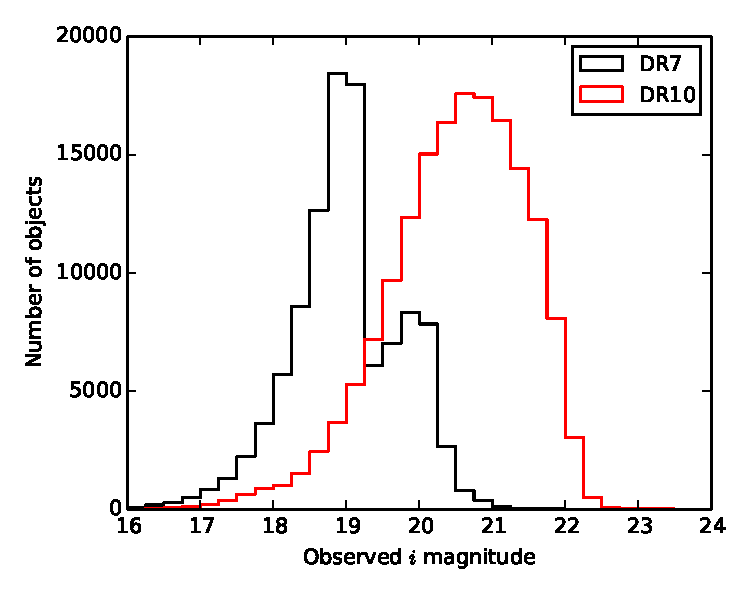
\includegraphics[width=\textwidth]{figures/chapter06/mihist}
  \end{minipage}\\ 
% \begin{minipage}[b]{0.5\textwidth}
%     \includegraphics[width=\textwidth]{figures/chapter06/Mihist} % can't find this file
%   \end{minipage}
  \caption{Histograms comparing the DR7Q and DR10Q catalogues: {\it Top:} Redshift distribution; {\it Middle:} Distribution of apparent $i$-band magnitudes; {\it Bottom:} Distribution of absolute $i$-band magnitudes {\bf missing this}.} 
  \label{fig:histograms}
\end{figure}

\subsection{UKIDSS Large Area Survey}

We use the UKIRT Infrared Deep Sky Survey \citep[UKIDSS;][]{lawrence07} Large Area Survey (ULAS) which has observed $\sim 3,200$ deg$^2$ in four near-IR passbands: $Y$ ($\lambda_{\rm eff} = 1.0305\mu$m), $J$ ($\lambda_{\rm eff} = 1.2483\mu$m), $H$ ($\lambda_{\rm eff} = 1.6313\mu$m), and $K$ ($\lambda_{\rm eff} = 2.2010\mu$m)). We used the ninth data release (DR9) of the ULAS. Cross-matching (with a 2$''$ radius and picking only the nearest neighbour) the SDSS DR7Q catalogue with the ULAS catalogue, which covers only $\sim 38$\% of the SDSS foot-print, resulted in 37,893 matches. The ULAS magnitudes are aperture corrected magnitudes in a 2$''$ diameter aperture and are not corrected for Galactic extinction.

UKIDSS fluxes and their associated errors are included in the DR10Q catalogue. These were converted to Vega magnitudes using flux zero points $2026$, $1530$, $1019$, and $631$ $\times10^{-26}$ W m$^{-2}$ Hz$^{-1}$ for the $Y$, $J$, $H$, and $K$ passbands respectively. Vega magnitudes were then converted to the AB system using the conversions given in Table \ref{tab:magconversions}. The UKIDSS fluxes in the DR10Q catalogue were obtained via forced photometry of UKIDSS observations at the SDSS DR8 centroids \citep{aihara11}. This method underestimates the intrinsic magnitude, as flux which falls outside of the aperture used is unaccounted for. We estimated the correction required to recover the intrinsic magnitudes by finding the median magnitude offset between the sub-sample of objects which have both UKIDSS DR10Q magnitudes and magnitudes from our SDSS DR7Q match to the ULAS DR9 catalogue, which is aperture corrected. We found the median offsets in the $Y$-, $J$-, $H$- and $K$- bands to be $-0.083$, $-0.081$, $-0.085$ and $-0.085$ respectively, and so corrected all DR10Q UKIDSS magnitudes by these amounts. 

\begin{table}
  \centering
  \begin{tabular}{c c c}
    \hline
    Band-pass & $m_{\rm Vega} \rightarrow m_{\rm AB}$ \\
    \hline \\
    $Y$ & $+0.634$ \\
    $J$ & $+0.938$ \\
    $H$ & $+1.379$ \\
    $K$ & $+1.900$ \\
    $W1$ & $+2.699$ \\
    $W2$ & $+3.339$ \\
    $W3$ & $+5.174$ \\
    $W4$ & $+6.620$ \\
    \hline
  \end{tabular}
  \caption{Vega to AB magnitude conversion factors for UKIDSS \citep{hewett06} and WISE \citep{cutri13} photometry.}
  \label{tab:magconversions}
\end{table}

\subsection{WISE All-WISE Survey}

The Wide-field Infrared Explorer \citep[WISE;][]{wright10} mapped almost the sky in four mid-IR band-passes: $W1$ ($\lambda_{\rm eff} = 3.4\mu$m), $W2$ ($\lambda_{\rm eff} = 4.6\mu$m), $W3$ ($\lambda_{\rm eff} = 12\mu$m), and $W4$ ($\lambda_{\rm eff} = 22\mu$m). The WISE AllWISE Data Release (`AllWISE') combines data from the nine month cryogenic phase of the mission that led to the `AllSky' data release with data from the NEOWISE program \citep{mainzer11}. 

Cross-referencing the SDSS DR7Q catalogue with the AllWISE catalogue resulted in 102,734 matches. Two objects (SDSS J083746.57+085839.6 and SDSS J092021.93+331125.7) were matched to multiple AllWISE objects, and were discarded from the sample. Cross-referencing the SDSS DR10Q catalogue with the AllWISE catalogue produced 116,666 matches. Four objects (SDSS J165812.28+3109000.6, SDSS J013053.17+034934.5, SDSS J151446.14+304241.8, and SDSSJ015615.57+034604.4) were matched to multiple AllWISE objects, and were discarded from the sample. 


\section{Completeness of Photometry}

We can set the brightness of our sample of quasars by excluding all objects with observed $i$ or $g$ magnitudes fainter than $i_{\rm min}$ or $g_{\rm min}$. Objects which are very bright in the $i$ or $g$ band-passes will also be detected at longer wavelengths. However, objects which are fainter in the $i$ or $g$ band-passes are more likely to have magnitudes which fall below the limiting magnitudes of the UKIDSS and WISE band-passes, and so will not be detected at these longer wavelengths. For a given $i$ or $g$ magnitude, a quasar with a blue spectrum (i.e. a spectrum which is fainter than usual at longer wavelengths) is more likely to be undetected at longer wavelengths than a quasar with a red spectrum (i.e. a spectrum which is brighter than usual at longer wavelengths). Therefore, as we allow fainter quasars in to our sample we will be biased towards objects with redder spectra. We can avoid this bias by carefully selecting the minimum $i$ or $g$ magnitude of the sample such that a large fraction (e.g. $\sim$95\%) of objects are detected in all band-passes and the fraction is not changing rapidly with the brightness of the sample (which would indicate we are close to the limiting magnitude of the survey). Figure \ref{fig:completeness} shows the fraction of objects which were matched to the SDSS DR7Q/DR10Q catalogue and have WISE and UKIDSS photometry with S/R $>$ 5 as a function of the minimum observed $i$/$g$ magnitude for the DR7Q/DR10Q sample. S/N ratios were calculated using

\begin{eqnarray}
  {\rm S/R} = \left( 0.4 \times {\rm log}(10) \times \sigma_m \right)^{-1}
\end{eqnarray}

where $\sigma_m$ is the uncertainty in the magnitude. We see that the DR7Q-matched sample is 95\% complete in all band-passes (excluding $W3$) if the minimum $i$ magnitude of the sample is above $\sim 20$. The DR10Q-matched sample is $\sim$ 95\% complete in all band-passes (again, excluding $W3$) if the minimum $g$ magnitude of the sample is above $\sim 20.5$. 

\begin{figure}
  \centering
  \begin{minipage}[b]{0.75\textwidth}
    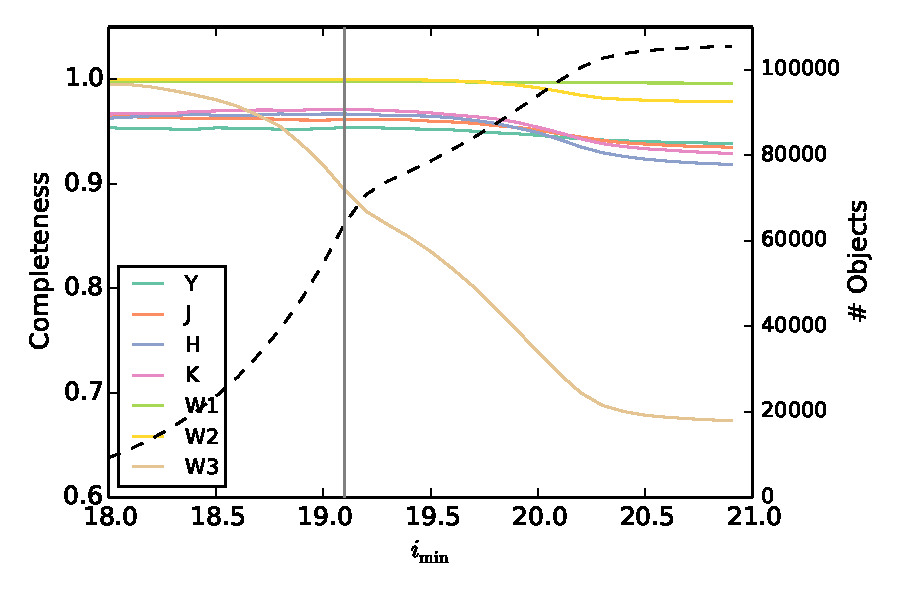
\includegraphics[width=\textwidth]{figures/chapter06/dr7completeness_v2}
  \end{minipage} \\
  \begin{minipage}[b]{0.75\textwidth}
    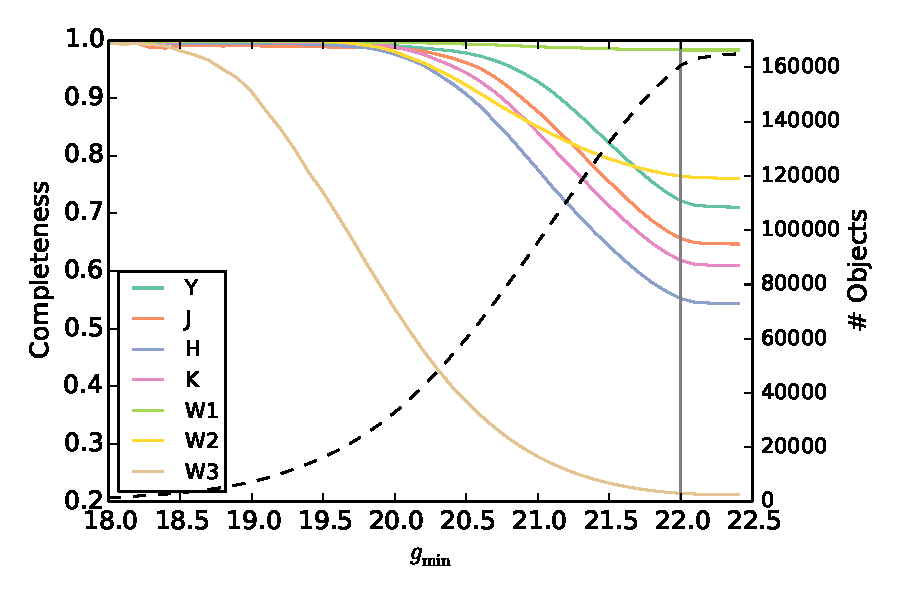
\includegraphics[width=\textwidth]{figures/chapter06/dr10completeness_v2}
  \end{minipage}
  \caption{{\it Top:} Fraction of objects which were matched to DR7Q catalogue with WISE and UKIDSS photometry (SNR $>$ 5) as a function of minimum $i$-band magnitude of the sample ({\it coloured lines}). Total number of objects in DR7Q catalogue as function of minimum $i$-band magnitude ({\it black dashed line}). Primary quasar colour selection minimum $i$ magnitude ({\it grey line}). {\it Bottom:} Fraction of objects which were matched to DR10Q catalogue with WISE and UKIDSS photometry (SNR $>$ 5) as a function of minimum $g$-band magnitude of sample ({\it coloured lines}). Total number of objects in DR10Q catalogue as function of minimum $g$-band magnitude ({\it black dashed line}). Primary quasar colour selection minimum $g$ magnitude ({\it grey line}).}
  \label{fig:completeness}
\end{figure}

In this chapter, we have described how we have constructed two large multi-wavelength quasar samples, one matched to the SDSS DR7Q catalogue and the other matched to the SDSS DR10Q catalogue. In addition to 13-band photometry we have moderate resolution spectra from SDSS in the $\sim 3000 - 9000$\AA~ region. We will use the spectra to complement our SED fitting by measuring, for example, SMBH masses, metallicities, and properties of absorbers and outflows.  

\newpage

\section{SED Model}
\label{chapter:sedmodel}

\begin{figure}[h]
  \centering
  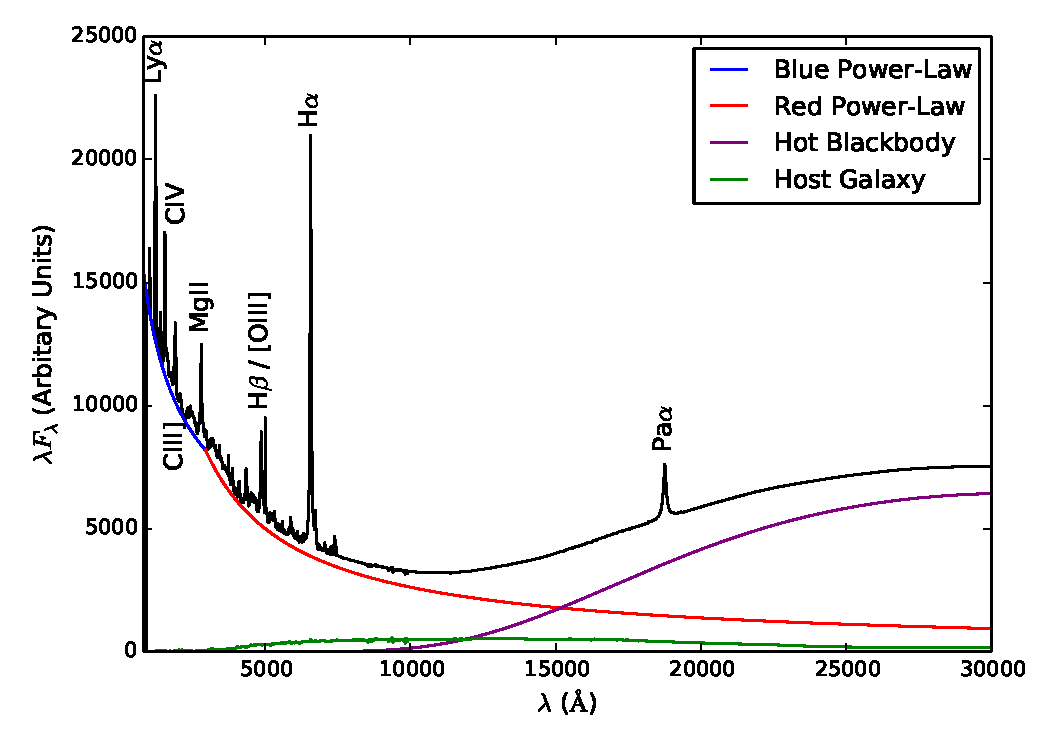
\includegraphics[width=\textwidth]{figures/chapter06/modelsed}
  \caption{Model spectrum at $z=1$, showing the contributions to the total flux from the blue power-law slope, red power-law slope, blackbody and host galaxy. The locations of the most prominent emission lines in the spectrum are also indicated. }
  \label{fig:modelsed}
\end{figure}

I have constructed a new SED model which attempts to reproduce the SEDs of AGNs from the rest-frame UV ($\sim 0.1 \mu$m) to the rest-frame near-IR ($\sim 3 \mu$m). In this chapter, I will describe how I have modelled the emission from the various components contributing to the emission in this spectral region. The model spectrum is shown in Figure \ref{fig:modelsed}, with each of the main components indicated. 

\section{Model Components}

\subsection{Accretion Disk}

As we described in Section \ref{sec:sed}, more than half the bolometric luminosity of an unobscured AGN is emitted in the Big Blue Bump, which extends from the near-IR at 1 $\mu$m to past 0.1 $\mu$m in the UV, and possibly all the way to the soft X-ray region (see Figure \ref{fig:seyfert_sed}), and is thought to arise from an accretion disc. In the 0.1 - 1 $\mu$m region the spectrum is generally characterised by a power-law of the form $F_\nu = C\nu^{-\alpha}$ where $\alpha$ is the power-law index, $C$ is a constant, and $F_\nu$ is the flux per unit frequency, usually measured in units of erg s$^{-1}$ cm$^{-2}$ Hz$^{-1}$. Equivalently this can be expressed as $F_\lambda = C^\prime\lambda^{\alpha - 2}$ where $F_\lambda$ is the flux per unit wavelength, usually measured in units of s$^{-1}$ cm$^{-2}$ \AA$^{-1}$. 

The value of the power-law index is uncertain. From a theoretical perspective, models of geometrically thin accretion discs \citep{shakura73} assume, in particular, that the disc is stationary, axisymmetric, and extends down to the innermost stable circular orbit, and that angular momentum is transported by local `viscous' stresses that convert gravitational energy entirely into heat. This gives the dependence of the effective temperature on radius as $t_{\rm eff} \propto r^{-3/4}$. A spectrum is then calculated by dividing the disc into concentric annuli, calculating the spectrum emitted by each annulus and then summing them all together. Assuming that each annulus radiates like a blackbody, the $r^{-3/4}$ effective temperature distribution gives $F_\nu \propto \nu^{1/3}$ \citep{peterson95}, although it is unclear whether this is consistent with observations.    

In our model we characterised the Big Blue Bump from $\sim 0.1 - 1 \mu$m as a broken power-law with three free parameters: a break-wavelength $\lambda_{\rm break}$, a blue power-law index $\alpha_{\rm blue}$ for wavelengths shorter than the break wavelength, and a red power-law index $\alpha_{\rm red}$ for wavelengths longer than the break wavelength.   

\subsection{Hot Dust}

At wavelengths longer than $1\mu$m, emission from hot dust begins to dominate over emission from the accretion disc. The SED in this region is generally characterised either by a power-law ($\propto \lambda^{\beta_{\rm NIR}}$), with $\beta \simeq 0.5$ \citep[e.g.][]{richards06, zhang14}, or by a blackbody at $\sim 1300$ K, thus peaking in the near-IR \citep[e.g.][]{leipski14}. We modelled the hot dust emission using a simple blackbody:

\begin{eqnarray}  
  F_\lambda =\frac{2 hc^2}{\lambda^5}\frac{1}{ e^{\frac{hc}{\lambda k_\mathrm{B}T}} - 1} 
\end{eqnarray}

The blackbody component has two free parameters: the temperature of the blackbody $T_{\rm BB}$ and the overall normalisation. 
 
\subsection{Emission Lines}

Hundreds of emission lines are present in a typical AGN spectra. Some of the most prominent lines are shown in Figure \ref{fig:modelsed}. The emission line spectrum is taken from \citet{maddox06}, who extend the composite of \citet{francis91} to include the H$\alpha$ (6560\AA) and Pa$\alpha$ (18750\AA) emission lines. A single parameter, EL$_{\rm scale}$, scales the equivalent widths of all emission lines equally:

\begin{eqnarray}
  F_{\lambda} =  {\rm EL}_{\rm scale} \times \frac{F_{\lambda, \rm el}}{F_{\lambda, \rm cont}} \times F_{\lambda} 
\end{eqnarray} 

where $F_{\lambda, \rm el}$ is the line flux in the template, $F_{\lambda,\rm cont}$ is the continuum flux in the template, and $F_{\lambda}$ is the continuum flux in the model.  

\subsection{Host Galaxy}

Emission from the host galaxy is important, particularly in the region around the $1\mu$m inflection point in the quasar SED. While the host galaxies of bright quasars tend to be massive, bright ellipticals, the hosts of lower luminosity AGN can have disc components \citep[e.g.][]{dunlop03}. Our model incorporates $z=0$ Sa, Sb, Sc and elliptical-type templates from \citet{mannucci01}, which for simplicity do not evolve with redshift. We characterise the relationship between the luminosity of the AGN $L_{\rm AGN}$ and the luminosity of the host galaxy $L_{\rm Gal}$ as a power-law

\begin{eqnarray}
  \label{eq:lgal}
  L_{\rm Gal} = L_{\rm AGN}^{\beta} 
\end{eqnarray}

with power-law index $\beta=0.42$ \citep{maddox06}. Dividing both sides of Equations \ref{eq:lgal} by the luminosity of the AGN gives the luminosity of the host galaxy relative to the luminosity of the AGN

\begin{eqnarray}
  \frac{L_{\rm Gal}}{L_{\rm AGN}} = L_{\rm AGN}^{\beta - 1} 
\end{eqnarray}

which for $\beta < 1$ decreases with increasing AGN luminosity. In a flux limited sample, the AGN luminosity will tend to increase with redshift and so the luminosity of the host galaxy relative to the luminosity of the quasar will decrease with increasing redshift. Hence, the contribution from the host galaxy to the total flux is important at low redshift, but becomes gradually less significant towards higher redshifts. 

Since the contribution from the host galaxy to the flux changes as a function of AGN luminosity, and hence redshift, we choose a reference redshift $z_{\rm nrm}$ where we set the fractional contribution of the host galaxy to the total flux, $\eta$. In an arbitrary region of the spectrum (we use $4000 - 5000$ \AA) we calculate both the AGN continuum flux $F_{\rm AGN}(z_{\rm nrm})$ and the flux from our host galaxy template spectrum $F_{\rm Gal}(z_{\rm nrm})$. The fractional contribution from the host galaxy to the total flux is then:

\begin{eqnarray}
  \label{eq:eta}
  \eta = \frac{CF_{\rm Gal}(z_{\rm nrm})}{F_{\rm AGN}(z_{\rm nrm}) + CF_{\rm Gal}(z_{\rm nrm})}
\end{eqnarray}

where the constant $C$ is the factor by which we must multiply the unnormalised galaxy spectrum in order for Equation \ref{eq:eta} to hold true. Rearranging for the constant $C$ we find

\begin{eqnarray}
  C = \frac{\eta}{1 - \eta} \frac{F_{\rm AGN}(z_{\rm nrm})}{F_{\rm Gal}(z_{\rm nrm})}
\end{eqnarray}
 
Hence at redshift $z_{\rm nrm}$ the host galaxy flux we add to our rest frame quasar continuum is 

\begin{eqnarray}
  \label{eq:flambda}
  F_{\lambda} = \frac{\eta}{1 - \eta} \frac{F_{\rm AGN}(z_{\rm nrm})}{F_{\rm Gal}(z_{\rm nrm})} F_{\lambda,{\rm Gal}}
\end{eqnarray}

where $F_{\lambda,{\rm Gal}}$ is our host galaxy template spectrum in the quasar rest frame. The contribution from the host galaxy at a different redshift $z$ is given by  

\begin{eqnarray}
  F_{\lambda} & = & \frac{\eta}{1 - \eta} \frac{F_{\rm AGN}(z)}{F_{\rm Gal}(z)} \frac{F_{\rm AGN}(z_{\rm nrm})}{F_{\rm Gal}(z_{\rm nrm})} \left( \frac{F_{\rm AGN}(z)}{F_{\rm Gal}(z)} \right)^{-1}  F_{\lambda,{\rm Gal}} \\ 
& = &  \frac{\eta}{1 - \eta} \frac{F_{\rm AGN}(z)}{F_{\rm Gal}(z)} \frac{F_{\rm AGN}(z_{\rm nrm})}{F_{\rm Gal}(z_{\rm nrm})}  \frac{F_{\rm Gal}(z)}{F_{\rm AGN}(z)}   F_{\lambda,{\rm Gal}} \\ & = &  \frac{\eta}{1 - \eta} \frac{F_{\rm AGN}(z)}{F_{\rm Gal}(z)} \frac{L_{\rm AGN}(z_{\rm nrm})}{L_{\rm Gal}(z_{\rm nrm})}  \frac{L_{\rm Gal}(z)}{L_{\rm AGN}(z)}  F_{\lambda,{\rm Gal}}  \\ & = & \frac{\eta}{1 - \eta} \frac{F_{\rm AGN}(z)}{F_{\rm Gal}(z)} \frac{L_{\rm AGN}(z_{\rm nrm})}{L_{\rm AGN}(z_{\rm nrm})^\beta}  \frac{L_{\rm AGN}(z)^\beta}{L_{\rm AGN}(z)}  F_{\lambda,{\rm Gal}} \\ & = &  \frac{\eta}{1 - \eta} \frac{F_{\rm AGN}(z)}{F_{\rm Gal}(z)} \left( \frac{L_{\rm AGN}(z)}{L_{\rm AGN}(z_{\rm nrm})} \right)^{\beta - 1}  F_{\lambda,{\rm Gal}}
\end{eqnarray}

We need to know how the luminosity of the AGN depends on redshift. This is given by:

\begin{eqnarray}
  \frac{L_{\rm AGN}(z)}{L_{\rm AGN}(z_{\rm nrm})} = 10^{-0.4(M_{\rm AGN}(z)-M_{\rm AGN}(z_{\rm nrm}))}
\end{eqnarray}

where $M_{\rm AGN}(z)$, the absolute magnitude of an AGN at redshift $z$, is given by

\begin{eqnarray}
  M(z) = m - 5({\rm log_{10}}D_{\rm L}(z) - 1)
\end{eqnarray}

and $D_{\rm L}(z)$ is the luminosity distance to a source at redshift $z$ in parsecs. Hence:

\begin{eqnarray}
  \frac{L_{\rm AGN}(z)}{L_{\rm AGN}(z_{\rm nrm})} & = & 10^{-0.4(M_{\rm AGN}(z)-M_{\rm AGN}(z_{\rm nrm}))} \\
  & = & 10^{({\rm log_{10}} \left( \frac{D_{\rm L}(z)}{D_{\rm L}(z_{\rm nrm})} \right)^2 )}
\end{eqnarray}
 

\subsection{Lyman-$\alpha$ Forest Absorption}

The optical spectra of high redshift quasars show hundreds of sharp absorption lines, which mostly correspond to the redshifted neutral hydrogen Ly$\alpha$ 1216\AA~transition. These absorption features are collectively referred to as the {\it Lyman-$\alpha$ forest}. To simulate the effect of Lyman-$\alpha$ forest absorption on our model SED we use the parametrisation of \citet{becker13}, who derived an analytic function for the effective optical depth $\tau_{\rm eff}$ over the redshift range 2 $< z <$ 5 made using 6065 quasar spectra from SDSS DR7. In their model the effective optical depth $\tau_{\rm eff}$ is given by 

\begin{eqnarray}
  \label{eq:taueff}
  \tau_{\rm eff} & = & \tau_0 \times ( \left( \frac{ 1 + z }{ 1 + z_0 } \right)^b + C )
\end{eqnarray}

where,

\begin{eqnarray*}
  t_0 & = & 0.751 \\
  b & = & 2.9 \\
  C & = & -0.132 \\
  z_0 & = & 3.5 
\end{eqnarray*}

The transmitted flux $F_{\lambda,{\rm trans}}$ at redshift $z$ is then given by 

\begin{eqnarray}
  \label{eq:ftrans}
  f_{\lambda,{\rm trans}} = F_\lambda \times e^{ -\tau_{\rm eff} }
\end{eqnarray}

An absorption line at $\lambda_{\rm abs}$ in the rest-frame of an AGN at redshift $z_{\rm AGN}$ has wavelength 

\begin{eqnarray}
  (1 + z_{\rm AGN})\lambda_{\rm abs} 
\end{eqnarray}

in the rest frame of an observer on Earth. In the rest-frame of a cloud of neutral hydrogen at redshift $z_{\rm cloud}$ the absorption line has wavelength 

\begin{eqnarray}
  \frac{ (1 + z_{\rm AGN}) \lambda_{\rm abs} } { (1 + z_{\rm cloud}) }
\end{eqnarray}

and so to absorb Lyman-$\alpha$ at 1216 \AA~ the gas cloud must be at a redshift

\begin{eqnarray}
  \label{eq:zcloud}
  z_{\rm cloud} = \frac{ (1 + z_{\rm AGN}) \lambda_{\rm abs} } { 1216{\rm \AA} } - 1
\end{eqnarray}

For every wavelength $\lambda_{\rm abs} < 1216$ \AA~ in the rest-frame of an AGN at redshift $z > 2$ we calculate $z_{\rm cloud}$ using Equation \ref{eq:zcloud} and then calculate the transmitted flux at $\lambda_{\rm abs}$ by substituting $z_{\rm cloud}$ in to Equations \ref{eq:taueff} and \ref{eq:ftrans}. 

\subsection{Lyman-Limit Systems}

{\it Lyman-limit systems} are clouds of HI which are optically thick at the Lyman limit ($912$\AA), which generally implies a neutral hydrogen column density $N(HI) > 10^{17} {\rm cm}^{-2}$. Photons at wavelengths shorter than the Lyman-limit will be absorbed, which creates a sharp break in the observed continuum. We model the effect of a Lyman-limit system at the redshift of the quasar by setting the flux at wavelengths less that 912\AA~ in the quasar rest frame to zero.   

\subsection{Dust Extinction} 

The selection criteria of the SDSS DR7Q catalogue, and particularly the DR10Q catalogue, are sensitive to quasars with moderate amounts of dust reddening \citep[possibly as high as E(B-V) $\sim$ 0.5;][]{richards03} at the redshift of the quasar, and so we included the effect of dust extinction in our model. We considered four types of extinction curve: the Large Magellanic Cloud (LMC), Small Magellanic Cloud (SMC), Milky-Way (MW) extinction curves from \citet{pei92} and an extinction curve appropriate for the quasar population which has been derived by Paul Hewett. To derive the quasar extinction curve, UKIDSS photometry was used to provide an E(B-V) estimate, via the magnitude displacement of each quasar from the locus of unreddened objects. At redshifts $2 < z < 3$ the reddening measure is made at rest-frame wavelengths 3500-7000\AA, where Galaxy, LMC and SMC extinction curves are very similar. The SDSS spectra of the same objects are then employed to generate an empirical extinction curve in the ultraviolet, down to 1200\AA. The resulting curve has no 2200\AA~ feature and rises rapidly with decreasing wavelength but is not as steep as the SMC curve. The extinctions curves give the colour excess $E(B-\lambda)$ relative to the colour excess $E(B-V)$ as a function of wavelength $\lambda$. The colour excess $E(B-V)$ is related to the extinction in the $V$ band, $A(V)$, via a parameter $R$, 

\begin{eqnarray}
  A(V) = R \times E(B -V )
\end{eqnarray}

where $R = 3.1$ in the MW and $R \simeq 3$ in the Magellanic Clouds. Hence the extinction at a wavelength lambda $A(\lambda)$ is 

\begin{eqnarray}
  A(\lambda) = E(B-V) \times \left[ \frac{E(\lambda-V)}{E(B-V)} + R \right] 
\end{eqnarray}

where the colour excess $E(B-V)$ is a free parameter in our model. The attenuation of the flux at a given wavelength is then:

\begin{eqnarray}
  F_\lambda = F_\lambda10^{-A(\lambda)/2.5}
\end{eqnarray}

in the rest frame of the quasar. 

\section{Converting Spectrum into Observed SED}
\label{sec:sedconversion}

\begin{figure}
  \centering
  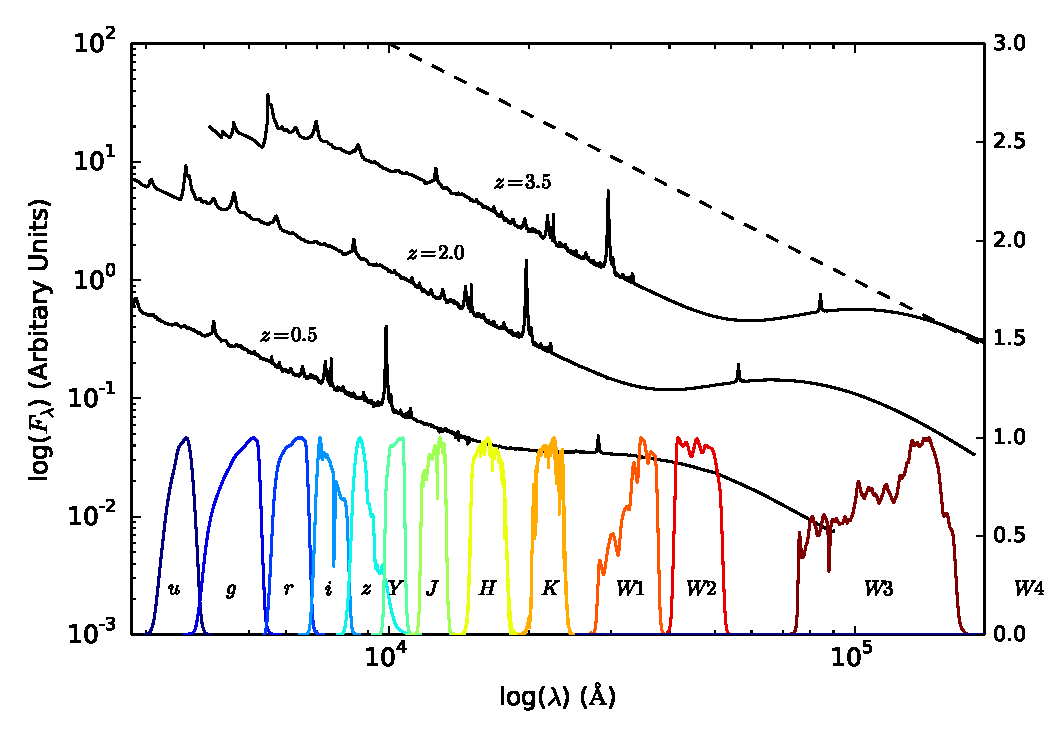
\includegraphics[width=\textwidth]{figures/chapter06/throughputs}
  \caption{Model spectrum at three different redshifts (each arbitrarily scaled), and throughput functions for SDSS, UKIDSS and WISE band-passes (scaled so that the peak transmission is equal to one.) The dashed line indicates the slope of the AB magnitude system zero point.}
  \label{fig:filters}
\end{figure}

The model spectrum was redshifted to the observed frame so that the apparent magnitude through each band-pass could be calculated. The throughput functions of the SDSS $ugriz$, UKIDSS $YJHK$ and WISE $W1W2W3$ band-passes are shown in Figure \ref{fig:filters}, along with our model AGN spectra at three different redshifts. The mean flux density in a band-pass P is given by 

\begin{eqnarray}
  \label{eq:flux}
  f_{\lambda}(P) & = & \frac{\int P(\lambda) f_\lambda(\lambda) \lambda d\lambda }{\int P(\lambda) \lambda d\lambda}
\end{eqnarray}

where $P(\lambda)$ is the dimensionless throughput function of the band-pass. The corresponding magnitude, $m_\lambda(P)$, is then 

\begin{eqnarray}
  m_\lambda(P) & = & -2.5{\rm log}(f_\lambda(P)) - m_0(P)
\end{eqnarray}

where $m_0(P)$ is the zero-point magnitude of band $P$. In the AB magnitude system, the zero-point flux per unit wavelength is 

\begin{eqnarray}
  \frac{f_\lambda(\lambda)}{{\rm erg}~{\rm cm}^{-2}~{\rm s}^{-1} {\rm\AA}^{-1}} = 0.1087 \left(\frac{\lambda}{\rm \AA}\right)^{-2} .
\end{eqnarray}

This is substituted into Equation \ref{eq:flux} to give a zero-point mean flux density which is then converted into a corresponding magnitude.  

\newpage

\section{Results From Fit} 
\label{chapter:results}

\section{Fitting Procedure}

In this chapter, we will describe the results of fitting our model to the SEDs of different samples of quasars. We will begin by deriving a `standard' SED model by constraining a single set of parameters with a large sample of $0.2 < z < 4$ quasars encompassing a range of luminosities, accretion rates etc. We will then go on to study the diversity of SED shapes in our quasar sample. In particular, we will search for the most heavily reddened quasars in the sample and also explore the redshift dependence of the hot dust properties of individual quasars. 

\subsection{The `Standard' SED Model} 

We use our SDSS DR7Q-matched sample which, as we saw in Figure \ref{fig:histograms}, is more complete over a wider redshift range than the DR10Q-matched sample. We impose an observed $i$ magnitude lower limit of 19.1 mag, which is the magnitude limit of the main SDSS colour-selection algorithm. We also exclude the objects flagged as BALQSOs by \citet{shen11}, since our model is unable to reproduce the broad absorption troughs that appear in the spectra of these objects. The final sample contains 61,411 objects in the redshift range $0.2 < z < 3.8$. 

The free parameters in our model are the blue power-law slope, the red power-law slope, the power-law break wavelength, the blackbody temperature, the blackbody normalisation, the emission line equivalent width scaling, and the fractional contribution from the host galaxy to the total flux. The reddening E(B-V) is fixed to zero, since a large fraction of SDSS quasars have very small amounts of dust reddening \citep{richards03}. For the host galaxy we use a Sb-type template derived by \citet{mannucci01}. With some choice of initial parameters, we generate a set of model observed spectra at redshifts from $z=0.25$ to $z=3.75$ in intervals of $\Delta z = 0.1$. We then transform our set of model spectra into a set of model $ugrizYJHKW1W2$ SEDs using the procedure described in Section \ref{sec:sedconversion}, which we normalise such that the $i$ magnitude of each model SED is 18.0 mag. This gives us an array of model magnitudes as a function of redshift and band-pass. We generate an equivalent data array by dividing our quasar sample into redshift bins from $z=0.2$ to $z=3.8$ with bin width $\Delta z = 0.1$. We normalise the individual quasar SEDs such that the observed $i$ magnitude is equal to 18.0 mag, and then calculate a median SED in each redshift bin. 

To fit the model to the data we minimise the sum of the squares of the differences between the elements in the model magnitude array and the elements in the data magnitude array. The minimisation is done using the `nelder-mead' method (also known as the downhill simplex method or amoeba method), as implemented in the {\tt minimize} function from the Python module {\tt scipy}. Our SED model is valid only up to $\lambda \sim 3\mu$m in the quasar rest frame (the approximate wavelength of the peak in hot dust emission); beyond this additional contributions to the total flux from cooler dust will become significant. This prevents us from using the two highest wavelength WISE bands in the fit. We also exclude the SDSS $u$ and $g$ band-passes from the fit at $z > 2.7$ and $z > 3.7$ respectively, where absorption in the Lyman$\alpha$ forest becomes large. 

The best-fitting parameters from the fit are shown in Table \ref{tab:params}. The colours ($u - g$, $g - r$, etc.) of the median SED, the individual quasars, and the best-fitting model are plotted as a function of redshift in Figure \ref{fig:colorplots}.  Most of the large variations that can be seen in the median colours of the quasars as a function of redshift are due to strong emission lines being redshifted in to and out of the bandpasses of the band-passes being used. 

% In Figure \ref{bandfits} we show the number of objects contributing to the median in each bandpass in each redshift bin. Change this if can to move maximum redshift to 4. 

% \begin{figure}
%   \centering
%   \begin{minipage}[b]{0.75\textwidth}
%   \includegraphics[width=\textwidth]{dr7bandfits}
% \end{minipage} \\
% \begin{minipage}[b]{0.75\textwidth}
%   \includegraphics[width=\textwidth]{dr10bandfits}
%   \end{minipage}
%   \caption{Number of magnitudes contributing to median in each redshift bin. $i$- and $Y$- bands are representative of all other bands in SDSS and UKIDSS respectively. Number of magnitudes contributing to median in each redshift bin in fit to DR10 sample. $i$- and $Y$- bands are representative of all other bands in SDSS and UKIDSS respectively.}
%   \label{fig:bandfits}
% \end{figure}

\begin{table}
  \centering
  \begin{tabular}{c c c c}
    \hline 
    Parameter & Symbol & Before Correction & After Correction \\
    \hline 
    Blue power-law index & $\alpha_{\rm blue}$ & 0.58 & 0.58 \\
    Red power-law index & $\alpha_{\rm red}$ & -0.04 & -0.05 \\
    Power-law break & $\lambda_{\rm break}$ & 2945 & 2957 \\
    Blackbody temperature & $T_{\rm BB}$ & 1216 K & 1186 K \\
    Blackbody normalisation & $C_{\rm BB}$ & 0.22 & 0.21 \\
    Emission line scaling & $C_{\rm EL}$  & 0.63 &  0.73 \\
    Galaxy fraction & $\eta$ & 0.29 & 0.28 \\
    E(B-V) & E(B-V) & 0.00 & 0.00 \\
    \hline
  \end{tabular}
  \caption{Best-fitting parameters from fit to DR7Q-matched sample.}
  \label{tab:params}
\end{table}

% using paul's rest frame range. no dust correction. 
% {'plslp2': [(0.68, -0.04086615936349667), (0.0, -0.030179914733468038), (0.68, -0.019491110272311915)], 'plslp1': [(0.68, 0.5560920143911354), (0.0, 0.566445634151032), (0.68, 0.5769695865322066)], 'galfra': [(0.68, 0.2950772099187981), (0.0, 0.30242499993336269), (0.68, 0.30972644939580546)], 'elscal': [(0.68, 0.6852329585639878), (0.0, 0.71938921375186038), (0.68, 0.7544776329877738)], 'bbt': [(0.68, 1175.4120197214068), (0.0, 1186.0058268904836), (0.68, 1196.5362069917846)], 'plbrk': [(0.68, 2918.7684490551023), (0.0, 2953.3677924491926), (0.68, 2986.942733960554)], 'bbflxnrm': [(0.68, 0.20850629138021362), (0.0, 0.21150096293181914), (0.68, 0.21445163625904562)]}
% Power-law slope 1: 0.57
% Power-law slope 2: -0.03
% Power-law break wavelength: 2953.37
% Blackbody temperature: 1186.01
% Blackbody normalisation: 0.21
% Emission line scaling: 0.72
% Galaxy fraction: 0.30
% E(B-V): 0.00
% I-band Normalisation: 18.00

% Same, but SDSS extinction-corrected. 
% {'plslp2': [(0.68, -0.06297748855929068), (0.0, -0.052265693559787163), (0.68, -0.04168533463452541)], 'plslp1': [(0.68, 0.48438987490487206), (0.0, 0.4970593326401529), (0.68, 0.5096400020595849)], 'galfra': [(0.68, 0.22817247693442125), (0.0, 0.23706421522616183), (0.68, 0.2461017776170246)], 'elscal': [(0.68, 0.7937958386184585), (0.0, 0.83557784709799277), (0.68, 0.8770507586470674)], 'bbt': [(0.68, 1261.4280904809336), (0.0, 1274.9611308386832), (0.68, 1288.2870800975506)], 'plbrk': [(0.68, 2814.2663530814348), (0.0, 2849.9948367507272), (0.68, 2885.5498491565395)], 'bbflxnrm': [(0.68, 0.20658852373304928), (0.0, 0.20999332758648137), (0.68, 0.21331847314099417)]}
% Power-law slope 1: 0.50
% Power-law slope 2: -0.05
% Power-law break wavelength: 2849.99
% Blackbody temperature: 1274.96
% Blackbody normalisation: 0.21
% Emission line scaling: 0.84
% Galaxy fraction: 0.24
% E(B-V): 0.00
% I-band Normalisation: 18.00

% with flux correction:
% {'plslp2': [(0.68, -0.062382690214621235), (0.0, -0.053463837950980642), (0.68, -0.04480977506298902)], 'plslp1': [(0.68, 0.5612481249236522), (0.0, 0.56972765169469852), (0.68, 0.5782526098873766)], 'galfra': [(0.68, 0.27532081104216344), (0.0, 0.28165640126424946), (0.68, 0.2880968793020588)], 'elscal': [(0.68, 0.9328704112902197), (0.0, 0.9652527064170725), (0.68, 0.9971412754488724)], 'bbt': [(0.68, 1123.826325535705), (0.0, 1132.1171673784174), (0.68, 1140.242989393583)], 'plbrk': [(0.68, 2954.2602789609955), (0.0, 2982.2290077662738), (0.68, 3010.694442892571)], 'bbflxnrm': [(0.68, 0.2020469115699503), (0.0, 0.20468059603495059), (0.68, 0.20727254780672683)]}
% Power-law slope 1: 0.57
% Power-law slope 2: -0.05
% Power-law break wavelength: 2982.23
% Blackbody temperature: 1132.12
% Blackbody normalisation: 0.20
% Emission line scaling: 0.97
% Galaxy fraction: 0.28
% E(B-V): 0.00
% I-band Normalisation: 18.00
% \begin{figure}
%   \centering
%   \begin{minipage}[b]{0.49\textwidth}
%     \includegraphics[width=\textwidth]{colorplots_140709/ug.jpg}
%   \end{minipage}
%   \begin{minipage}[b]{0.49\textwidth}
%     \includegraphics[width=\textwidth]{colorplots_140709/gr.jpg}
%   \end{minipage} \\
% \begin{minipage}[b]{0.49\textwidth}
%     \includegraphics[width=\textwidth]{colorplots_140709/ri.jpg}
%   \end{minipage}
%   \begin{minipage}[b]{0.49\textwidth}
%     \includegraphics[width=\textwidth]{colorplots_140709/iz.jpg}
%   \end{minipage} \\
% \begin{minipage}[b]{0.49\textwidth}
%     \includegraphics[width=\textwidth]{colorplots_140709/zy.jpg}
%   \end{minipage}
%   \begin{minipage}[b]{0.49\textwidth}
%     \includegraphics[width=\textwidth]{colorplots_140709/yj.jpg}
%   \end{minipage} 
%   \caption{DR7 color redshift plots.}
%   \label{fig:color}
% \end{figure}

% \begin{figure}
%   \centering
%   \begin{minipage}[b]{0.49\textwidth}
%     \includegraphics[width=\textwidth]{colorplots_140709/jh.jpg}
%   \end{minipage}
%   \begin{minipage}[b]{0.49\textwidth}
%     \includegraphics[width=\textwidth]{colorplots_140709/hk.jpg}
%   \end{minipage} \\
% \begin{minipage}[b]{0.49\textwidth}
%     \includegraphics[width=\textwidth]{colorplots_140709/kw1.jpg}
%   \end{minipage}
%   \begin{minipage}[b]{0.49\textwidth}
%     \includegraphics[width=\textwidth]{colorplots_140709/w1w2.jpg}
%   \end{minipage} \\
% \begin{minipage}[b]{0.49\textwidth}
%     \includegraphics[width=\textwidth]{colorplots_140709/kw2.jpg}
%   \end{minipage}
%   \begin{minipage}[b]{0.49\textwidth}
%     \includegraphics[width=\textwidth]{colorplots_140709/hw1.jpg}
%   \end{minipage} 
%   \caption{DR7 color redshift plots continued.}
%   \label{fig:dr7color}
% \end{figure}

\begin{figure}
  \centering
  \begin{minipage}[b]{0.49\textwidth}
    \includegraphics[width=\textwidth]{figures/chapter06/sed_color_plots/ug.jpg}
  \end{minipage}
  \begin{minipage}[b]{0.49\textwidth}
    \includegraphics[width=\textwidth]{figures/chapter06/sed_color_plots/gr.jpg}
  \end{minipage} \\
\begin{minipage}[b]{0.49\textwidth}
    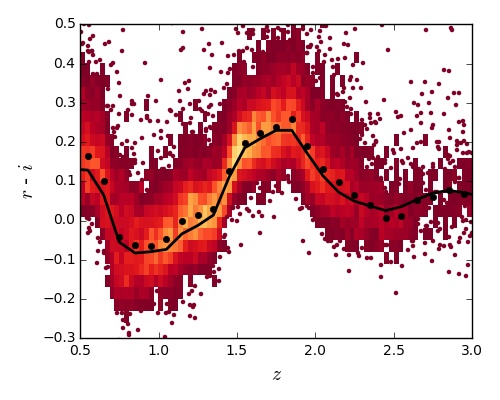
\includegraphics[width=\textwidth]{figures/chapter06/sed_color_plots/ri.jpg}
  \end{minipage}
  \begin{minipage}[b]{0.49\textwidth}
    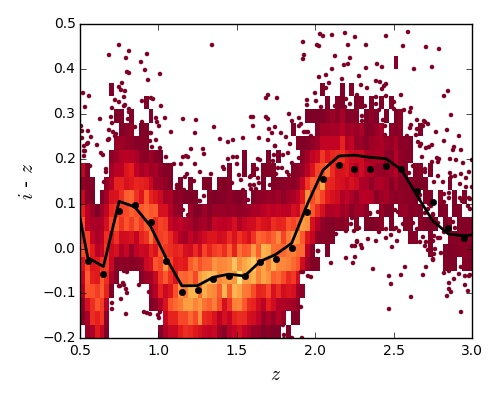
\includegraphics[width=\textwidth]{figures/chapter06/sed_color_plots/iz.jpg}
  \end{minipage} \\
\begin{minipage}[b]{0.49\textwidth}
    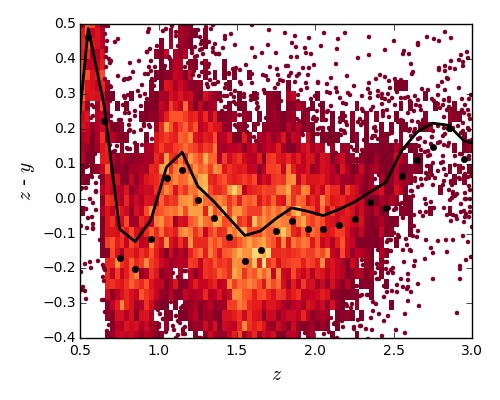
\includegraphics[width=\textwidth]{figures/chapter06/sed_color_plots/zy.jpg}
  \end{minipage}
  \begin{minipage}[b]{0.49\textwidth}
    \includegraphics[width=\textwidth]{figures/chapter06/sed_color_plots/yj.jpg}
  \end{minipage} 
\end{figure}

\begin{figure}
  \centering
  \begin{minipage}[b]{0.49\textwidth}
    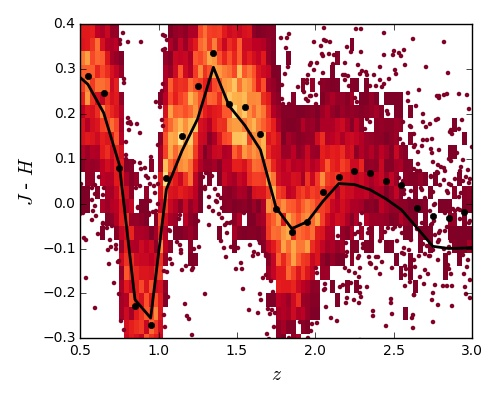
\includegraphics[width=\textwidth]{figures/chapter06/sed_color_plots/jh.jpg}
  \end{minipage}
  \begin{minipage}[b]{0.49\textwidth}
    \includegraphics[width=\textwidth]{figures/chapter06/sed_color_plots/hk.jpg}
  \end{minipage} \\
\begin{minipage}[b]{0.49\textwidth}
    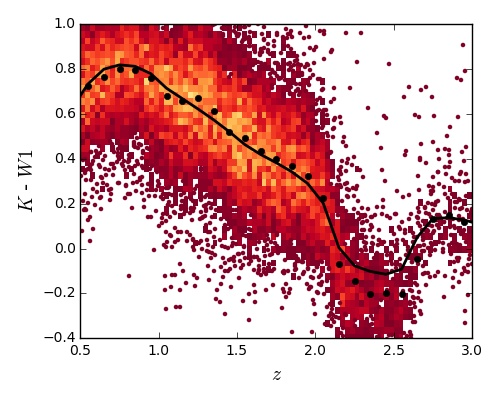
\includegraphics[width=\textwidth]{figures/chapter06/sed_color_plots/kw1.jpg}
  \end{minipage}
  \begin{minipage}[b]{0.49\textwidth}
    \includegraphics[width=\textwidth]{figures/chapter06/sed_color_plots/w1w2.jpg}
  \end{minipage} \\
\begin{minipage}[b]{0.49\textwidth}
    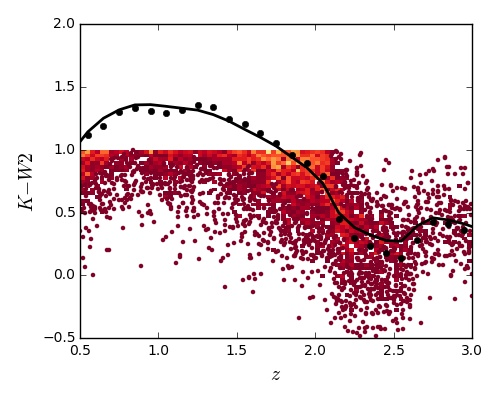
\includegraphics[width=\textwidth]{figures/chapter06/sed_color_plots/kw2.jpg}
  \end{minipage}
  \begin{minipage}[b]{0.49\textwidth}
    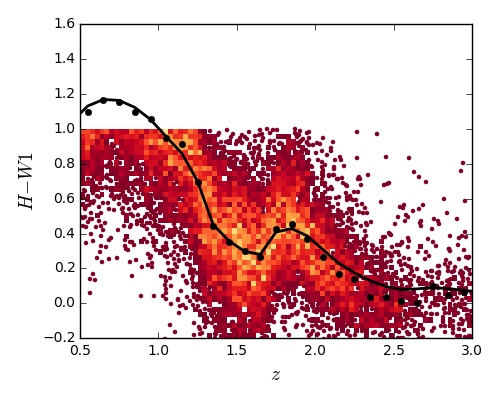
\includegraphics[width=\textwidth]{figures/chapter06/sed_color_plots/hw1.jpg}
  \end{minipage} 
  \caption{Colours of median SED ({\it black circles}), individual objects ({\it grey points}), best-fitting uncorrected model ({\it black line}) and best-fitting corrected model ({\it red line}) as a function of redsfit.}
  \label{fig:colorplots}
\end{figure}

% \begin{figure}
%   \centering
%   \begin{minipage}[b]{0.49\textwidth}
%     \includegraphics[width=\textwidth]{dr10colorplots/ug.jpg}
%   \end{minipage}
%   \begin{minipage}[b]{0.49\textwidth}
%     \includegraphics[width=\textwidth]{dr10colorplots/gr.jpg}
%   \end{minipage} \\
% \begin{minipage}[b]{0.49\textwidth}
%     \includegraphics[width=\textwidth]{dr10colorplots/ri.jpg}
%   \end{minipage}
%   \begin{minipage}[b]{0.49\textwidth}
%     \includegraphics[width=\textwidth]{dr10colorplots/iz.jpg}
%   \end{minipage} \\
% \begin{minipage}[b]{0.49\textwidth}
%     \includegraphics[width=\textwidth]{dr10colorplots/zy.jpg}
%   \end{minipage}
%   \begin{minipage}[b]{0.49\textwidth}
%     \includegraphics[width=\textwidth]{dr10colorplots/yj.jpg}
%   \end{minipage} 
%   \caption{fsdf}
%   \label{fig:color}
% \end{figure}

% \begin{figure}
%   \centering
%   \begin{minipage}[b]{0.49\textwidth}
%     \includegraphics[width=\textwidth]{dr10colorplots/jh.jpg}
%   \end{minipage}
%   \begin{minipage}[b]{0.49\textwidth}
%     \includegraphics[width=\textwidth]{dr10colorplots/hk.jpg}
%   \end{minipage} \\
% \begin{minipage}[b]{0.49\textwidth}
%     \includegraphics[width=\textwidth]{dr10colorplots/kw1.jpg}
%   \end{minipage}
%   \begin{minipage}[b]{0.49\textwidth}
%     \includegraphics[width=\textwidth]{dr10colorplots/w1w2.jpg}
%   \end{minipage} \\
% \begin{minipage}[b]{0.49\textwidth}
%     \includegraphics[width=\textwidth]{dr10colorplots/kw2.jpg}
%   \end{minipage}
%   \begin{minipage}[b]{0.49\textwidth}
%     \includegraphics[width=\textwidth]{dr10colorplots/hw1.jpg}
%   \end{minipage} 
%   \caption{fsdf}
%   \label{fig:color}
% \end{figure}

\subsection{Discussion of Fit}

\begin{figure}
  \centering
  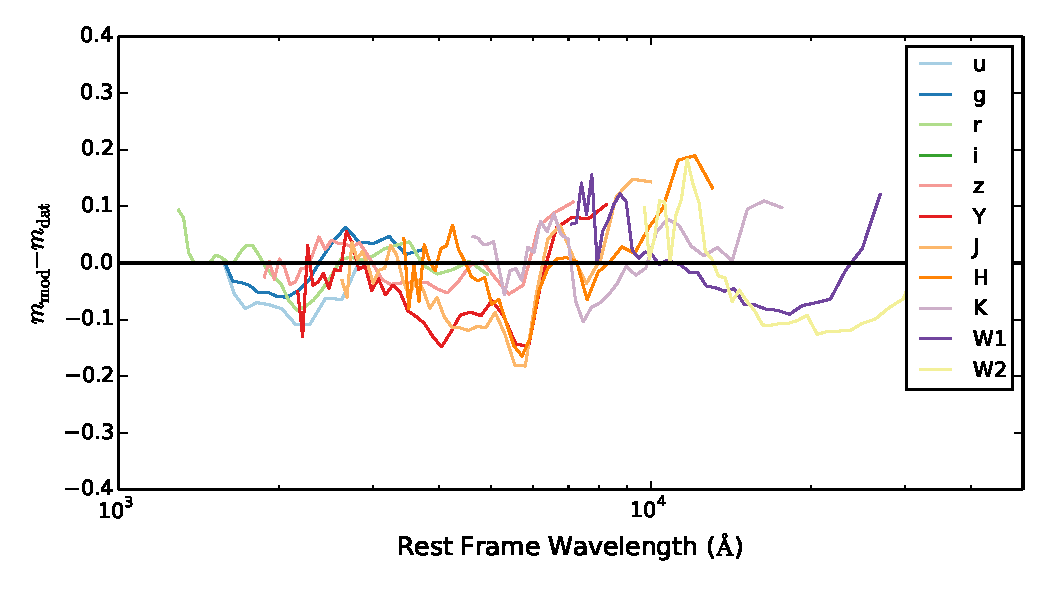
\includegraphics[width=\textwidth]{figures/chapter06/residuals_nocorr}
  \caption{Residuals from fit to DR7Q-matched catalogue as a function of rest-frame wavelength.}
  \label{fig:residuals}
\end{figure}

In Figure \ref{fig:residuals} we show the difference between the magnitudes from the best-fitting model and the median magnitudes from the sample. We have transformed the effective wavelengths of the band-passes to the rest frame of the quasars in each redshift bin, to give to the residuals as a function of rest-frame wavelength. In Figure \ref{fig:residuals} we represent the residuals measured in each band-pass using a different coloured line. Differences between residuals from different band-passes at the same rest-frame wavelength could indicate redshift evolution of the typical quasar SED. 

The residuals indicate that over a large redshift range the model does a fairly good at reproducing the median observed colours of the DR7Q-matched sample. Most discrepancies are at the $<0.1$ mag level. 
It is remarkable that a single model is so effective; the properties of a typical quasar to not change significantly over a wide range of redshifts and luminosities. On the other hand, for the individual objects there is a significant scatter about the mean. In general, our goal is to use this intrinsic spread in SED properties in order to understand the diversity in physical quasar properties. 

The most noticeable feature in Figure \ref{fig:residuals} is a bump around 1$\mu$m, where the model underestimates the flux of the population by $\sim 0.1$ mag. Later on in Section \ref{sec:fluxcorrection} we will derive an empirical correction to the model which increases the flux slightly in the 8000 to 17000 \AA~ region of the rest frame spectrum. The red lines in Figure \ref{fig:colorplots} show the colours of this corrected model as a function of redshift. Although the correction improves the fit slightly, significant discrepancies do remain. The model's underestimation of the flux at in the 3$\mu$m region is probably due to the increasingly significant contribution to the flux from cooler dust at longer wavelengths, which is not included in our model. We will discuss this in more detail in Section \ref{sec:definingsample}. 

Our fitting scheme scales the equivalent width of every emission line by the same amount. Observationally, the emission line ratios are not the same for every quasar, and the model to data discrepancies in certain regions are likely to be the result of this. In Figure \ref{fig:residuals} we mark the position of the H$\alpha$ emission line, which is typically very strong and broad and can contribute significantly to the flux even in a broad band-pass. The relatively large residuals around the wavelength of the H$\alpha$ line may suggest that our simple scaling scheme is insufficient, and we may need to allow the equivalent widths of certain prominent emission lines to vary freely. 

\section{Reddened Quasars}
\label{sec:redobjects}

Having derived a `standard' SED model, we will now focus on a sub-sample of quasars with SEDs that are best fit by a standard model in addition to moderate amounts of dust reddening (0.1 $<$ E(B-V) $<$ 0.2). Numerous studies have identified quasars with extreme amounts of dust reddening; in this study it is our aim to first identify and then to study the properties of quasars with moderate amounts of dust reddening in order to understand the relationship between the extremely dust reddened and `normal' blue populations. Although heavily biased towards selecting blue, unobscured quasars, the SDSS is sensitive to quasars with dust reddening up to $E(B-V) \lesssim 0.5$ \citep{richards03}. 

\subsection{Colour Selection}

As we saw in Figure \ref{fig:colorplots}, quasar colours are a strong function of redshift, which is partly due to strong emission lines being shifted in to and out of the band-passes. Therefore, defining an object as `red' based on a colour cut is subject to redshift-dependent systematic errors. Instead, we calculate the $i-K$ colours of the quasars in the DR10Q-matched catalogue, which is deeper, and therefore more sensitive to reddened quasars, than the DR7Q-matched catalogue, relative to the $i-K$ colours of our standard SED model with E(B-V) = 0.0, 0.1, and 0.2. This is shown in Figure \ref{fig:ikvz}. Most of the DR10Q catalogue quasars lie in the $2 < z < 4$ redshift range in which both the SDSS $i$ band-pass and the UKIDSS $K$ band-pass are observing the UV/optical power-law spectrum, the shape of which is the most sensitive to dust reddening. We therefore restrict ourselves to the $2 < z < 4$ redshift range. Most of the scatter in the $i-K$ colours of the individual quasars can be attributed to variations in the power-law slope and emission line strength of individual objects from the standard model. However, there is also a population in the red tail of the distribution with colours that can only be explained by dust reddening at the redshift of the source \citep{hall04}. 

\begin{figure}
  \centering
  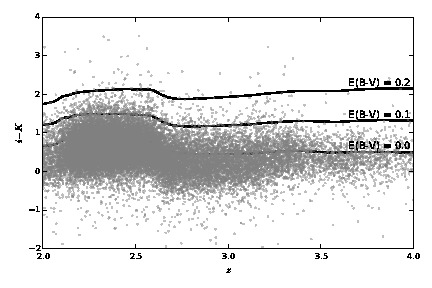
\includegraphics[width=\textwidth]{figures/chapter06/ikvz.jpg}
  \caption{$i-K$ colours of DR10Q-matched catalogue quasars as a function of redshift $z$ ({\it grey points}). $i - K$ colours of `standard' SED model as a function of redshift $z$ with dust reddening E(B-V)=0.0, 0.1, and 0.2 ({\it black lines}).}
  \label{fig:ikvz}
\end{figure}

We estimated an E(B-V) value for each object by interpolating between the reddened models in Figure \ref{fig:ikvz}. We selected a sample of 303 objects which have $i-K$ colours which are redder than the standard model with dust reddening E(B-V) = 0.2 (i.e. the grey points which lie above the top curve in Figure \ref{fig:ikvz}). We visually inspected the SDSS optical spectra of these objects and found a diverse range of properties. Approximately a third of the sample could be characterised visually as having reddened continuum emission. Many had very strong emission lines; some of these had normal blue continua and were probably included in the sample due strong H$\alpha$ emission in the $K$ band-pass. Up to $\sim 20\%$ were BALQSOs, and up to $\sim 10\%$ were Type II quasars. In Figure \ref{fig:spectra}, we show an example of an SDSS spectrum of an object we classified as being a reddened quasar (SDSS J150019.64+082643.6) and an example of an SDSS spectrum of an object which has very strong emission lines, but an otherwise normal blue continuum (SDSSJ 0240000.6+010317.0).  

\begin{figure}
  \centering
  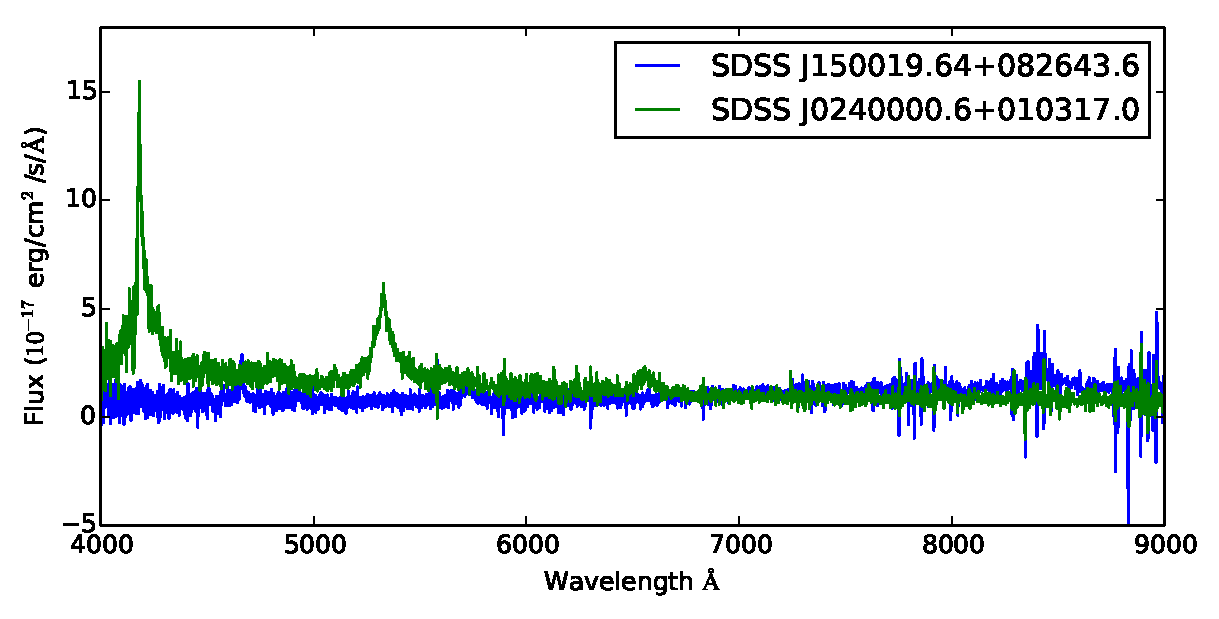
\includegraphics[width=\textwidth]{figures/chapter06/redspectra}
  \caption{SDSS spectra of two quasars with red $i-K$ colours relative to our unreddened SED model. Whereas the optical spectrum of SDSS J150019.64+082643.6 suggests it may be a genuinely dust-reddened quasar, the red colour of SDSS J0240000.6+010317.0 is probably due to strong H$\alpha$ emission in the $K$ band-pass.}
  \label{fig:spectra}
\end{figure}

\subsection{Model Fitting}

In order to select a sample of genuinely reddened quasars while excluding the strong emission line quasars that are contaminating our sample, we fit our model to the SEDs of the individual quasars. We are unable to constrain every parameter in our model with just 11 photometric data points, and so we fix all the parameters except the emission line strength and the dust reddening to the standard values we derived from the fit to the whole sample. To account for the dispersion of the colours of the individual quasars about the median line (see Figure \ref{fig:colorplots}) we set a minimum error of 0.1 mag on the magnitudes. Our model was fit to the data using a standard $\chi^2$ minimisation which, as before, was implemented using the `nelder-mead' algorithm as implemented in the {\tt minimize} module from the {\tt scipy} Python package with standard options. We used a larger sample of 3,117 quasars, which were selected to have $i-K$ colours above the E(B-V) = 0.1 dust reddened model in Figure \ref{fig:ikvz}. 

\begin{figure}
  \centering
  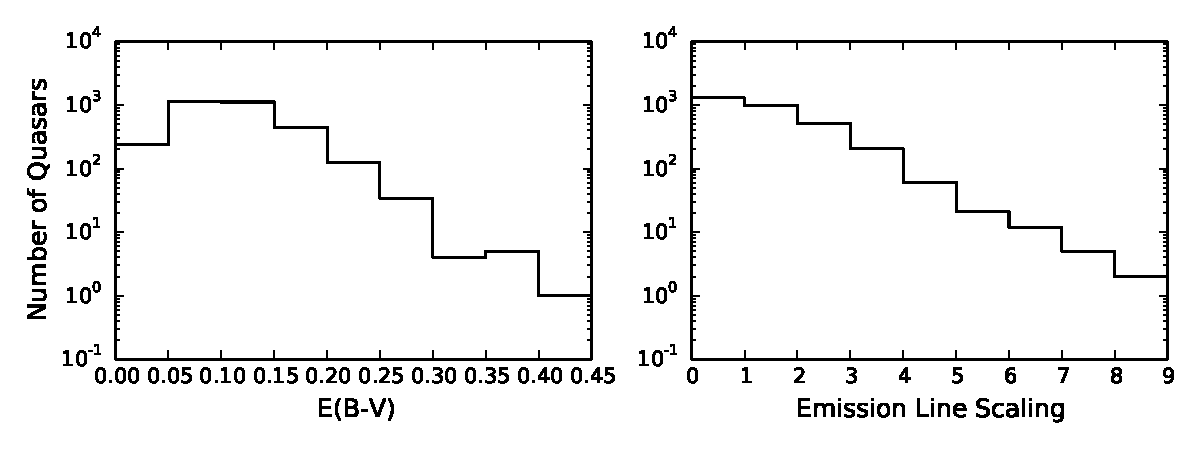
\includegraphics[width=\textwidth]{figures/chapter06/ebvandelscalhist}
  \caption{Dust reddening E(B-V) and emission line equivalent width distributions from SED fitting.}
  \label{fig:ebvelscalhist}
\end{figure}

In Figure \ref{fig:ebvelscalhist} we show the E(B-V) and emission line equivalent width scaling values we derived from the fit. The median dust reddening E(B-V) is 0.1, and the maximum is 0.61. 543 quasar SEDs were best fit by models with extremely weak emission lines (emission line equivalent width scaling parameter $< 0.01$). Of these quasars approximately 30\% were classified as BALQSOs. These objects have strong absorption troughs in their spectra which, when integrated over the wavelength range of a band-pass, could cancel out the emission line flux. However, visual inspection of the SDSS optical spectra of a sub-sample of the non-BALQSOs revealed the presence of significant emission lines when the best-fitting model suggested there should be none. In Figure \ref{fig:zhist_elscal} we show how the fraction of objects in the sample which are best fit by models with emission line equivalent width scaling parameter $< 0.01$ is a strong function of redshift, with significant peaks at $z \sim 2$ and $z \sim 2.7$. We interpret these peaks as being regions of redshift space for which strong emission lines do not affect the SED because they have been redshifted to wavelengths that are not probed by our set of band-passes. If we increase the emission line equivalent width scaling paramter to a value typical of the whole population (i.e. $\sim 0.8$), we find that the majority of $\chi^2$ values from the fit increase by less than one. This demonstrates that the parameter is not well constrained by the data; the emission lines can be of any strength without significantly changing the SED.   
 
\begin{figure}
  \centering
  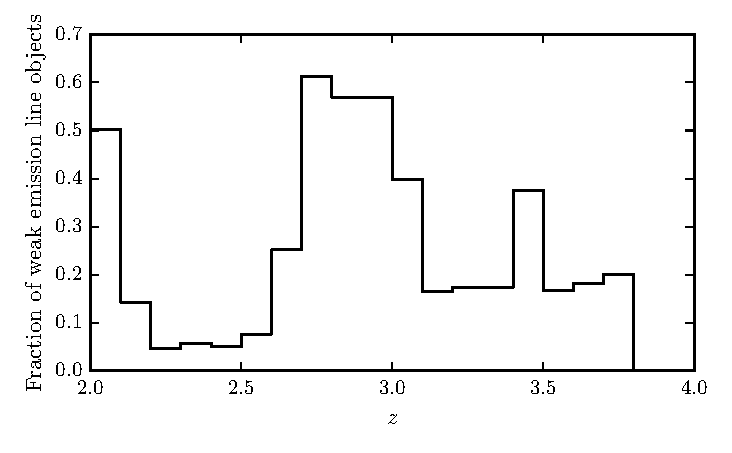
\includegraphics[width=\textwidth]{figures/chapter06/zhist_elscal}
  \caption{Fraction of quasars in 3,117 object sample which are best fit by models with emission line equivalent width scaling parameter $< 0.01$ as a function of redshift.}
  \label{fig:zhist_elscal}
\end{figure}

\subsection{MCMC Fitting}

We decided to address this limitation by imposing a prior on the emission line equivalent width scaling parameter. To do this we implemented a monte-carlo markov-chain (MCMC) fitting method using the Python module {\it pymc}. We determined a sensible prior on the emission line equivalent width scaling parameter by looking at the distribution of CIV equivalent widths in the DR10Q catalogue (excluding BALQSOs). We found that the equivalent width values were well fit by a lognormal distribution with location parameter $\mu = 3.737$ and scale parameter $\sigma = 0.58$. This motivated us to impose a lognormal prior on the emission line equivalent width scaling parameter with location parameter $\mu = 0$ and scale parameter $\sigma = 0.58$. We imposed uniform priors on the other two free parameters, the reddening E(B-V) and the overall normalisation of the spectrum. We our MCMC fits with 10,000 iterations and a burn-in length of 500. An example of a posterior plot for quasar SDSS J121956.49-011907.8 is shown in Figure \ref{fig:posteriorplot}. Some degeneracy between the parameters is evident, most obviously between the overall normalisation of the SED and the emission line equivalent width scaling. 

\begin{sidewaysfigure}
  \centering
  \includegraphics[width=\textwidth]{figures/chapter06/posteriorplot}
  \caption{Posterior plots from MCMC fit to SDSS J121956.49-011907.8.}
  \label{fig:posteriorplot}
\end{sidewaysfigure}

We found the mean E(B-V) values from the MCMC fit to be very similar to the best-fitting values from the $\chi^2$ fit (see Figure \ref{fig:ebvelscalhist}). The prior on the emission line equivalent width scaling parameter has ensured that we no longer have a significant population of objects which are incorrectly best-fit by models with very weak emission lines.

\subsection{Acquiring Near-IR Spectroscopy}

In the previous section we described how we have collected a sample of quasars with moderate amounts of dust reddening (E(B-V) $\lesssim$ 0.5) at the redshift of the quasar. The next stage in our investigation is to study the physical properties of these dust reddened objects, and to compare these to the properties of the population of unreddened quasars and the population of heavily reddened quasars \citep[e.g.][]{banerji12}. We are particulary interested in discovering how these populations are related. For example, are the moderately dust reddened quasars in our sample being observed as the quasar makes the transition from being heavily dust reddened to unobscured as it clears out its surrounding dust, or can their dust properties be explained in the context of orientation-based unification schemes.   

To help address this question, we plan to obtain near-IR spectra for a sub-sample of our moderately dust reddened quasars using the LIRIS instrument on the William Herschel Telescope at the Issac Newton Group of telescopes. For quasars in the redshift range $2 \lesssim z \lesssim 2.5$, the H$\alpha$ emission line should be observable using the $K$ band-pass on this instrument. The shape and width of this spectral line will provide us with information on the nature of the obscuring dust. For example, the presense of a broad component to the line would suggest that the dust extinction is occuring in the host galaxy rather than in a circum-nuclear torus, in which case the broad component should be obscured. The H$\alpha$ line properties can be used to infer black hole masses, bolometric luminosities, and Eddington ratios \citep{banerji12}, and these physical properties can then be compared to other populations.  

Due to the obvious constarints on obtainint telescope time, we needed to define a short-list of candidates for follow-up. To be a candidate we required the objects to pass the following criteria:

\begin{itemize}
\item Be viewable during the August - January observing window. 
\item Have a high S/N in the $K$ band-pass; the higher the S/N, the shorter the exposure time we will require. 
\item Be at a redshift $2 \lesssim z \lesssim 2.5$
\item Be well fit by the redenned standard SED model, with otherwise `normal' features, e.g. not a Type II quasar, BALQSO etc.  
\end{itemize}

Of the 3,117 quasars in our sample, 858 were obserable during the 1st August to 31st January observing semester\footnote{We made use of the on-line tool Staralt. Available at: http://catserver.ing.iac.es/staralt/index.php.}. Of these quasars, 567 were at redshifts for which the H$\alpha$ emission line will be observable in the $K$ band-pass ($2 \lesssim z \lesssim 2.5$). Of these, 252 were fit reasonably well by the standard model when the amount of dust reddening and the emission line equivalent width scaling strength were free to vary ($chi^2 \leq 10$). Of these, 19 quasars are brighter than 18 mag in the $K$ band-pass (for an object of this brightness we will require a $\sim 3000$s exposure to obtain a spectra with a S/R $\sim 10$\footnote{We made use of the LIRIS exposure time calculator. Available at: http://www.iac.es/proyecto/LIRIS/simulator/form\_LIRIS\_spect.html.}). The maximum amount of dust reddening E(B-V) (from our MCMC fit) in this sample of 19 quasars is 0.2, with 0.12 the median. Given the small number of objects in the sample with even modest amounts of reddening, we decided to delay the proposal untill the next observing semester, which runs from 1st February to 31st July. During this period 2.6 times as many objects will be observable, which should significantly increase the number of moderately reddened objects in the sample. 

\section{Hot Dust}

\begin{figure}
  \centering
  \begin{minipage}[b]{0.75\textwidth} 
    \includegraphics[width=\textwidth]{figures/chapter06/w1w2_bbt}
  \end{minipage} \\
  \begin{minipage}[b]{0.75\textwidth} 
    \includegraphics[width=\textwidth]{figures/chapter06/w1w2_bbflxnrm}
  \end{minipage}
  \caption{$W1 - W2$ colours of DR7 sample as a function of redshift, up to $z=1.8$. Above a certain density threshold points are represented by a density plot. On top we plot our standard model, with a blackbody temperature varying from 1000 - 1600 K ({\it top figure}) and a blackbody normalisation between 0 and 0.5 ({\it bottom figure}).}
  \label{fig:w1w2colors}
\end{figure}

In Figure \ref{fig:w1w2colors} we plot the $W1 - W2$ colors of the DR7Q-matched sample as a function of redshift from $z=0.2$ to $z=1.8$. In this redshift range the $W1$ and $W2$ band-passes are probing the 12,000 - 28,000 \AA~ and 16,000 - 38,000 \AA~ region of the rest frame SED respectively, and the $W1-W2$ color is therefore predominantly tracing emission from hot dust at temperatures $\sim 1200$ K. At any given redshift or, equivalently, region of the rest-frame SED, we see a $\sim 0.5$ mag dispersion in the $W1-W2$ colors. On the same axes in Figure \ref{fig:w1w2colors} we have plotted the $W1 - W2$ colors derived from our SED model with blackbody temperatures ranging from 1000 - 1600 K and blackbody normalisation factors (i.e. the flux from the blackbody component relative to the power-law continuum at a reference wavelength) from 0 - 0.5, with the other parameters as reported in Table \ref{tab:params}. A blackbody with a single temperature and normalisation is clearly not a very good representation of the hot dust properties of the whole sample. For example, dust which is futher from the accretion disc will be at a lower temperature, and if the covering factor of the dust around the accretion disc is smaller then the ratio of near-IR luminosity to UV/optical luminosity (which the blackbody normalisation is proportional to) will decrease. We aim to study the diversity hot dust properties of the quasars in our sample to learn about the nature of the hot dust, and to link the hot dust properties to other physical quantities such as the luminosity and redshift of the quasar. 

\subsection{Defining Sample}
\label{sec:definingsample}

We decided to explore the diversity of hot dust properties by fitting our standard model, with the blackbody temperature and normalisation as free paramters, to the individual quasar SEDs. The first step was to define a sample of quasars from the DR7Q-matched catalogue which were well fit by our standard un-reddened SED model. To achieve this we discarded from our sample quasars with $i - K$ colors redder than our standard model with dust reddening E(B-V) = 0.1 (see Figure \ref{fig:ikvz}). As we discussed in Section \ref{sec:redobjects}, this region of the $i-K$ colour space includes both quasars with significant amounts of dust redenning and quasars with extreme emission line equivalent widths. We exclude quasars with observed magnitudes fainter than 19.1 in the $i$ band-pass, as well as quasars with upper-limit or S/R $<$ 5 magnitudes in the $K$, $W1$ and $W2$ band-passes (without these we will be unable to properly constrain the blackbody slope). We exclude quasars flagged as BALQSOs from the sample, since these objects may be in a special evolutionary stage and have different hot dust properties (we will consider this in future work). Finally, from all of the objects which passed the above criteria, we discarded the 10\% of quasars which were least well fit by our standard model.   

It is important to consider the redshift range over which we can reasonably expect to be able to constrain the shape of the blackbody component. The amount by which the observed spectrum is redshifted determines the position of the hot dust feature in the spectrum relative to the wavelength coverage of our set of band-passes. For a redshift $z \sim 1.5$ quasar, only the $W2$ band-pass, at $\sim 2 \mu$m in the rest frame of the quasar, is probing the wavelength region dominated by the blackbody emission (the peak in a $T \sim 1200$K blackbody is at $\sim 2.4 \mu$m). At $z \gtrsim 1.5$, we found that we could no longer constrain the shape of the blackbody component in our SED model using the $ugrizYJHKW1W2$ band-passes. Although we could include magnitude constraints from the longer-wavelength WISE $W3$ band-pass ($\lambda_{\rm eff} \simeq 12 \mu$m), at $z \sim 1.5$ this is observing $\sim 5 \mu$m in the quasar's rest frame. In this region there will be extra contributions to the flux, possibly from cooler dust, which are not accounted for in our model. This was clearly demonstrated by the increase in the $m_{\rm model} - m_{\rm data}$ residuals beyond $\sim 3\mu$m in the rest frame. At lower redshifts, the $W3$ band-pass is probing even longer-wavelengths, where the component we are missing from our model will be greater. To compensate our SED model will move the blackbody component to lower temperatures, which shifts the peak to longer wavelengths. The result will be a downward trend in the blackbody temperature with decreasing redshift. Given that one question we are interested in addressing is variations in the hot dust properties with redshift, we have to be very wary of systematic effects such as these. With these considerations in mind, we restricted ourselves to determining the hot dust properties of our quasar sample in the redshift range $0.5 < z < 1.5$. 

\subsection{Flux Correction}
\label{sec:fluxcorrection}

In Figure \ref{fig:residuals} we saw how the model appeared to be underestimating the observed flux in the region around $1 \mu$m in the quasar rest frame spectrum. Since we are aiming to carefully constrain the shape of the blackbody component just long-ward of this wavelength region, we need to be very careful in how we deal with this discrepancy. A blackbody component with a higher temperature would contribute more flux in this region, which could potentially lead to redshift-dependent systemetatic errors very similar to those we have just described above. To avoid this we derived a correction to our model which accounted for the $1 \mu$m flux discrepency. 

\begin{figure}
  \centering
  \includegraphics[width=\textwidth]{figures/chapter06/residualscorrection}
  \caption{{\it Top:} Residuals from fitting the overall normalisation of the SED as a function of wavelength in the quasar rest frame. The different lines correspond to 101-point running medians for the $H$, $K$, $W1$ and $W2$ band-passes, and have been colour-coded to indicate the redshift for which the given quasar rest frame wavelength corresponds to the un-redshifted effective wavelength of the band-pass. The black line is a cubic interpolation of a 801-point running-median through through all residuals, irrespective of the band-pass used. The red dashed line marks the wavelength of the Pa$\alpha$ emission line. {\it Bottom:} The spectral model before and after the flux correction ({\it see main text}).}
  \label{fig:modelcorrection}
\end{figure}

We fit the overall normalisation of the model SED only; this is a constant vertical displacement we add to the model magnitudes. This fit is done in the 2000 - 9000 \AA~ region of the rest frame spectrum using our sample of `standard' quasars. We calculate the $m_{\rm data} - m_{\rm model}$ residuals for each quasar, and calculate the effective wavelength of each band-pass in the rest frame of the quasar. In Figure \ref{fig:modelcorrection} we show a 101-point running median through the residuals of each band-pass in the 6000 - 22000 \AA~ region of the quasar rest frame. The lines have been colour-coded to show the redshifts of the quasars which are contributing to the residuals in the corresponding region of the quasar rest frame. The black line in the Figure \ref{fig:modelcorrection} is a cubic interpolation of a 801-point running-median through all residuals as a function of the quasar rest frame wavelength, irrespective of the band-pass used. It shows quite clearly that the model is underestimating the observed flux over the $\sim 8,000 - 17,000$\AA~ rest frame wavelength region. We calculated the multiplicative factor which when applied to the model spectrum accounted for the model to data magnitude discrepancy, i.e. the amount of flux `missing' from the model. In the bottom panel of Figure \ref{fig:modelcorrection} we show our model spectrum both with and without this correction term. In Figure \ref{fig:colorplots} we show how the fit is imporved in the $\sim 1\mu$m region of the rest frame spectrum.  

\section{Results From Blackbody Fit}

We fixed the overall normalisation of the quasar SEDs to values from the 2000 - 9000 \AA~ fit, and fit for the temperature and normalisation of the blackbody component in the 10,000 - 23,000 \AA~ region of the rest frame spectrum (i.e. the spectral region most sensitive to hot dust emission). In Figure \ref{fig:bbtvz} we show the best-fitting blackbody temperature for the quasars in our sample as a function of redshift. The solid lines are running-medians through the points, calculated both before and after we applied the correction to the model described in the preceding section. The difference is stark; after we apply the flux correction the median best-fitting blackbody temperature drops by $\sim 200$K to $\sim 1200$K. This is encouraging, since 1200K is the best-fitting blackbody temperature from the fit to the whole DR7Q-matched sample. Although we see no significant evolution of the hot dust properties in this redshift range, we plan to test this at higher redshift. We will also compare the hot dust properties of interesting subpopulations (e.g. Type II quasars, BALQSOs) and look for correlations with physical parameters of the quasar (e.g. luminosity, Eddington ratio). 

\begin{figure}
  \centering
  \includegraphics[width=\textwidth]{figures/chapter06/bbt_z.pdf}
  \caption{Blackbody temperature from fit against redshift before correction ({\it grey circles}). Black line is running median through blackbody temperatures before correction, blue line is running median after correction.}
  \label{fig:bbtvz}
\end{figure}

\newpage

\section{Conclusions and Future Work}

While many authors have focused on studies of specific sub-sets of AGN with extreme observational properties, what is missing is an understanding of how these extreme subsets relate to the population as a whole. In particular, we will focus on merger-based scenarios for quasar/galaxy co-evolution, which predict an obscured growth phase before the enshrouding dust is blown out, and schemes which explain the variety of observational properties as being only apparent differences due to non-spherical source geometries. We will study this issue by combining large-area photometric surveys from SDSS, UKIDSS and WISE. Multi-wavelength surveys allow us to gain a more holistic view of quasar properties by sampling their entire SED. We have a developed a model to fit the quasar SED in the 1 - 3 $\mu$m spectral region which, at present, can constrain the following features:

\begin{itemize}
\item {\bf Power-law slope}, which relates to properties of the accretion disk.
\item {\bf Blackbody temperature and normalisation}, which relates to properties of circum-nuclear hot dust. 
\item {\bf Dust Reddening}, at redshift of quasar, which relates to dust properties of the quasar and its host galaxy. 
\item {\bf Emission line strength}, which relates to properties of emission line regions and absorbing dust. 
\end{itemize}

The SDSS DR10Q catalogue, which was made available in late 2013, contains $\sim 120,000$ quasars at $z\gtrsim2$ ($\sim$ 5 times the number previously known). This will allow us to study quasar properties at the epoch when quasar activity peaked. Crucially, moderate-resolution optical spectra are available for all sources in the SDSS catalogue, which will allow us to relate SED properties to, for example, the black-hole mass and properties of outflowing gas. There is also the possibility, at least for a sub-set of objects, of extending our multi-wavelength SED coverage using data from, for example, FIRST in the radio and Spitzer in the far-IR. 

\subsubsection{Specific Investigations}

\subsubsection{Hot Dust Properties}

The near-IR excess in the SED is believed by many to be emission from dust at its sublimation temperature at the inner edge of a torus structure. We are able to test this by linking properties of the hot dust (e.g. the luminosity) to other properties of the quasar (e.g. bolometric luminosity, redshift). For example, is there any evidence for the inner edge of the torus being further from the nucleus in more luminous quasars (i.e. a decrease in near-IR to optical/UV luminosity ratio with increasing optical/UV luminosity)? Are there quasars in our sample which are deficient in hot dust and, if so, are these objects being observed before a dusty torus has formed or are the torus and accretion disk misaligned? 

\subsubsection{E(B-V) Distribution}

Deriving the dust-reddening E(B-V) distribution of our optically selected sample will allow us to relate the small samples of extremely reddened objects which have been found to the population of mildly reddened quasars. Are these extreme objects in the tail of a population of mildly reddened quasars or are there equal distributions of mildly reddened and extremely reddened quasars? A similar analysis was done by \citet{richards03}, but with the DR10Q catalogue we are able to pick up far more objects during the peak epoch when both quasar activity and star-formation rates peaked ($2 \lesssim z \lesssim 4$). Obtaining near-IR spectra for a sample of moderately reddened quasars will give us crucial information about the level and scale of the dust extinction. We will also use our sample to derive a new extinction curve appropriate for the quasar population.

\subsubsection{BALQSOs}

Broad, blue-shifted absorption lines are associated with AGN-driven out-flowing gas, and outflows are a key component in galaxy evolution models with AGN feedback. With an adapted model, we will derive information from the SED (e.g. the dust-reddening) which, when combined with outflow properties measured in the SDSS spectra, will allow us to study the population of BALQSOs in relation to the population as a whole. Are BALQSOs observed during a special `blow-out' phase in a quasars lifetime, or is outflowing gas only detected along certain sight-lines? 

\subsubsection{Type II Quasars}

How are the population of obscured Type II quasars related to the Type I population? Does the Seyfert Type I/II dusty-torus unification scheme extend to higher luminosities or are Type II quasars observed in a special phase of quasar growth? Again, properties derived from the multi-wavelength SEDs and optical spectra will help to relate these objects to the population as a whole. 


\section{Draft Paper}

\section{Introduction}

Understanding the link between supermassive black-hole growth and the properties of Active Galactic Nuclei (AGN) host galaxies is one of the most important areas of galaxy-formation research. It is now well established that non-spherical geometries including some form of obscuring material on parsec scales (possibly in the form of a torus), can explain much of the observed diversity seen in the spectral energy distributions (SEDs) of AGN. At the same time, AGN-driven outflows are present in a large fraction of the luminous quasar population. The mass and energy associated with these outflows is believed to be significant in the context of feedback and its effect on the host galaxy. Punctuated fuelling episodes, e.g. driven by galaxy mergers, satellite accretion and even secular processes, almost certainly lead to AGN experiencing activity-, outflow- and obscuration-dominated cycles with some overlap between phases. Quantitatively, however, it remains unclear how these phases relate to the fundamental properties of the accreting black-hole (e.g.  mass (M$_{\rm{BH}}$), bolometric luminosity (L$_{\rm{bol}}$) and Eddington ratio (L/L$_{\rm{Edd}}$) and the elements of the non-spherical geometry). 

With large-scale surveys from SDSS, UKIDSS, and {\it WISE} providing information on the SEDs covering rest-frame 0.1-3.0\,$\mu$m wavelengths for thousands of AGN at redshifts $2 \lesssim z \lesssim 3$ it is finally possible to study the link between outflow diagnostics from ultra-violet spectra, e.g. as measured from the C\,{\sc iv} emission line, and emission from hot (T $\simeq$ 1200K) dust peaking in the NIR, which provides information about the amount and geometry of gas and dust on parsec scales. In one model, quasars are surrounded by an inner `wall' of gas and dust, in a cylinder-like geometry. As a radiatively-driven outflow develops, material at the extremes of the cylinder is driven-off, exposing more of the inner edge of the obscuring material at the equator (a `torus'), which contains the hot dust. Quasars are also observed with a wide distribution of reddening from dust on galactic scales. It is believed that luminous highly dust-reddened quasars may be in the process of expelling their dust and transitioning to  ultra-violet bright objects  which make up to the majority of the SDSS sample.

\section{Data}

The systematic study of the dependence of the SED shape on physical parameters has, until very recently, been limited by the difficulty in obtaining a large sample of quasars with good multi-wavelength coverage and large dynamic range in luminosity and redshift. In this work, we take advantage of a number of recent, sensitive, wide-field surveys, covering the UV to mid-IR spectral region. 

We use the spectroscopic quasar catalogues of the Sloan Digital Sky Survey \citep[SDSS;][]{york00} Seventh Data Release \citep[DR7Q;][]{schneider10} and Tenth Data Release \citep[DR10Q;][]{paris14}. DR7Q and DR10Q include 105,783 objects across 9380 deg$^2$, and 166,583 objects across 6,370 deg$^2$, respectively, with 16,420 objects in common to both catalogues. The SDSS obtained images in five broad optical passbands: $u$ ($\lambda_{\rm eff} = 3543$\AA), $g$ ($\lambda_{\rm eff} = 4770$\AA), $r$ ($\lambda_{\rm eff} = 6231$\AA), $i$ ($\lambda_{\rm eff} = 7625$\AA), and $z$ ($\lambda_{\rm eff} = 9134$\AA). The SDSS spectra cover $\sim 3000 - 9000$\AA~ at a spectral resolution of $\sim 2000$. We use BEST point-spread function (PSF) magnitudes from the DR7Q catalogue, correcting for Galactic extinction using the maps of \citet{schlegel98}, assuming a Milky Way (MW) extinction curve \citep{pei92} and an extinction to reddening ratio ${\rm A}(V) / {\rm E}(B-V) = 3.1$. We use the PSF magnitudes from the DR10Q catalogue, correcting for Galactic extinction using the maps of \citet{schlafly11}. Although the SDSS asinh magnitude system is intended to be on the AB system \citep{oke83}, the photometric zero-points are known to be slightly off the AB standard. To account for this we add 0.03 mag to the $u$, $g$, $r$ and $i$ magnitudes, and 0.05 mag to the $z$ magnitude.  

We use the UKIRT Infrared Deep Sky Survey \citep[UKIDSS;][]{lawrence07} Large Area Survey (ULAS) which has observed $\sim 3,200$ deg$^2$ in four near-IR passbands: $Y$ ($\lambda_{\rm eff} = 1.0305\mu$m), $J$ ($\lambda_{\rm eff} = 1.2483\mu$m), $H$ ($\lambda_{\rm eff} = 1.6313\mu$m), and $K$ ($\lambda_{\rm eff} = 2.2010\mu$m)). We used the ninth data release (DR9) of the ULAS. Cross-matching (with a 2$''$ radius and picking only the nearest neighbour) the SDSS DR7Q catalogue with the ULAS catalogue, which covers only $\sim 38$\% of the SDSS foot-print, resulted in 37,893 matches. The ULAS magnitudes are aperture corrected magnitudes in a 2$''$ diameter aperture and are not corrected for Galactic extinction. UKIDSS fluxes and their associated errors are included in the DR10Q catalogue. These were converted to Vega magnitudes using flux zero points $2026$, $1530$, $1019$, and $631$ $\times10^{-26}$ W m$^{-2}$ Hz$^{-1}$ for the $Y$, $J$, $H$, and $K$ passbands respectively. Vega magnitudes were then converted to the AB system using the conversions given by \citet{hewett06}. Mention correction? 

The Wide-field Infrared Explorer \citep[WISE;][]{wright10} mapped almost the sky in four mid-IR band-passes: $W1$ ($\lambda_{\rm eff} = 3.4\mu$m), $W2$ ($\lambda_{\rm eff} = 4.6\mu$m), $W3$ ($\lambda_{\rm eff} = 12\mu$m), and $W4$ ($\lambda_{\rm eff} = 22\mu$m). The WISE AllWISE Data Release (`AllWISE') combines data from the nine month cryogenic phase of the mission that led to the `AllSky' data release with data from the NEOWISE program \citep{mainzer11}. Cross-referencing the SDSS DR7Q catalogue with the AllWISE catalogue resulted in 102,734 matches. Cross-referencing the SDSS DR10Q catalogue with the AllWISE catalogue produced 116,666 matches. 

\section{UV Spectra Parameters}

\section{Model Description}

\begin{figure}
  \centering
  \includegraphics[width=\columnwidth]{figures/chapter06/modelsed}
  \caption{Model spectrum at $z=1$, showing the contributions to the total flux from the blue power-law slope, red power-law slope, blackbody and host galaxy. The locations of the most prominent emission lines in the spectrum are also indicated. }
  \label{fig:modelsed}
\end{figure}

Our model aims to reproduce the SEDs of AGNs from the rest-frame UV ($\sim 0.1 \mu$m) to the rest-frame near-IR ($\sim 3 \mu$m). The model spectrum is shown in Figure \ref{fig:modelsed}, with each of the main components indicated. We characterise the Big Blue Bump from $\sim 0.1 - 1 \mu$m as a broken power-law with three free parameters: a break-wavelength $\lambda_{\rm break} = 2822\AA$, a blue power-law index $\alpha_{\rm blue} = 0.46$ for wavelengths shorter than the break wavelength, and a red power-law index $\alpha_{\rm red} = 0.03$ for wavelengths longer than the break wavelength. At wavelengths longer than $1\mu$m, emission from hot ($T \simeq 1200$K) dust begins to dominate over emission from the accretion disc. We modelled the hot dust emission using a simple blackbody:

\begin{eqnarray}  
  F_\lambda =\frac{2 hc^2}{\lambda^5}\frac{1}{ e^{\frac{hc}{\lambda k_\mathrm{B}T}} - 1} 
\end{eqnarray}

Hundreds of emission lines are present in a typical AGN spectra. Some of the most prominent lines are shown in Figure \ref{fig:modelsed}. The emission line spectrum is taken from \citet{maddox06}, who extend the composite of \citet{francis91} to include the H$\alpha$ (6560\AA) and Pa$\alpha$ (18750\AA) emission lines. A single parameter, EL$_{\rm scale}$, scales the equivalent widths of all emission lines equally:

\begin{eqnarray}
  F_{\lambda} =  {\rm EL}_{\rm scale} \times \frac{F_{\lambda, \rm el}}{F_{\lambda, \rm cont}} \times F_{\lambda} 
\end{eqnarray} 

where $F_{\lambda, \rm el}$ is the line flux in the template, $F_{\lambda,\rm cont}$ is the continuum flux in the template, and $F_{\lambda}$ is the continuum flux in the model.  

Emission from the host galaxy is important, particularly in the region around the $1\mu$m inflection point in the quasar SED. While the host galaxies of bright quasars tend to be massive, bright ellipticals, the hosts of lower luminosity AGN can have disc components \citep[e.g.][]{dunlop03}. Our model incorporates $z=0$ Sa, Sb, Sc and elliptical-type templates from \citet{mannucci01}, which for simplicity do not evolve with redshift. We characterise the relationship between the luminosity of the AGN $L_{\rm AGN}$ and the luminosity of the host galaxy $L_{\rm Gal}$ as a power-law $L_{\rm Gal} = L_{\rm AGN}^{\beta}$ with power-law index $\beta=0.42$ \citep{maddox06}.

To simulate the effect of dust extinction at the redshift of the quasar we used an extinction curve appropriate for the quasar population. To derive the quasar extinction curve, UKIDSS photometry was used to provide an E(B-V) estimate, via the magnitude displacement of each quasar from the locus of unreddened objects. At redshifts $2 < z < 3$ the reddening measure is made at rest-frame wavelengths 3500-7000\AA, where Galaxy, LMC and SMC extinction curves are very similar. The SDSS spectra of the same objects are then employed to generate an empirical extinction curve in the ultraviolet, down to 1200\AA. The resulting curve has no 2200\AA~ feature and rises rapidly with decreasing wavelength but is not as steep as the SMC curve. 

\subsection{Sample}

We selected quasars from the SDSS DR7 catalogue. We included only quasars targeted by the main quasar selection algorithm (i.e. $i < 19.1$), and quasars classified by ?? as lacking broad (width < something) absorption troughs. Furthermore, we excluded quasars with S/N < 5.0 in the $K$, $W1$, and $W2$ passbands. After fits, excluded 10\% of outliers. 

\begin{figure}
  \centering
  \includegraphics[width=\columnwidth]{figures/chapter06/ikzplot}
  \caption{$i-K$ vs $z$. Demonstrates how sample was defined. The grey points show, as a function of redshift, the $i-K$ colours of all DR7Q quasars which are not classified as broad-absorption line quasars by Shen et al. and $i$ magnitude > 19.1. The black line shows the $i-K$ colour of our standard, unreddened SED model as a function of redshift. The red and blue lines show the $i-K$ colours of our SED model with dust reddening E(B-V) = 0.075 and E(B-V) = -0.075 respectively. A significant amount of this reddening can be attributed to intrinsics variations in the UV power-law slopes of the indidual quasars, which is why we allow a negative reddening. However, there is a clear `red tail' to the colour distribution which can be explained by dust reddending at the redshift of the quasar. We definined two samples, at low ($0.5 < z < 1.5$) and high ($2 < z < 2.7$) redshift, which are shown in the figure.}
  \label{fig:ikzplot}
\end{figure}

\section{Results}

\section{Hot Dust}

\begin{figure}
\centering
\includegraphics[width=\columnwidth]{figures/chapter06/w1w2_z_v2}
\caption{$W1 - W2$ colours of DR7 sample as a function of redshift, up to $z=1.8$. Above a certain density threshold points are represented by a density plot. On top we plot our standard model, with a blackbody temperature varying from 1000 - 1600 K ({\it top figure}) and a blackbody normalisation between 0 and 0.5 ({\it bottom figure}). Around $z=1.5$ the model no longer appears to be a very good fit to the data, which I suppose is just the fact that the blackbody is turning over, whereas in the data the flux keeps incresing (additional contributions from cooler components.) Add ticks to top of top panel. Think about how useful these plots really are. In top plot I'm changing the temperature, which is changing the normalisation (Lum IR). This is effectively same as bottom plot, except here I'm keeping the shape the same, just moving it up and down. Even if this is fine these plots are probably a bit misleading as they are (need to be clear normalisation will also be changing in the top plot.}
  \label{fig:w1w2colors}
\end{figure}

In Figure \ref{fig:w1w2colors} we plot the $W1 - W2$ colors of the DR7Q-matched sample as a function of redshift from $z=0.2$ to $z=1.8$. In this redshift range the $W1$ and $W2$ band-passes are probing the 12,000 - 28,000 \AA~ and 16,000 - 38,000 \AA~ region of the rest frame SED respectively, and the $W1-W2$ color is therefore predominantly tracing emission from hot dust at temperatures $\sim 1200$ K. At any given redshift or, equivalently, region of the rest-frame SED, we see a $\sim 0.5$ mag dispersion in the $W1-W2$ colors. On the same axes in Figure \ref{fig:w1w2colors} we have plotted the $W1 - W2$ colors derived from our SED model with blackbody temperatures ranging from 1000 - 1600 K and blackbody normalisation factors (i.e. the flux from the blackbody component relative to the power-law continuum at a reference wavelength) from 0 - 0.5, with the other parameters as reported in Table \ref{tab:params}. A blackbody with a single temperature and normalisation is clearly not a very good representation of the hot dust properties of the whole sample. We aim to study the diversity hot dust properties of the quasars in our sample to learn about the nature of the hot dust, and to link the hot dust properties to other physical quantities such as the luminosity and redshift of the quasar. 

We decided to explore the diversity of hot dust properties by fitting our standard model, with the blackbody temperature and normalisation as free paramters, to the individual quasar SEDs. 

The first step was to define a sample of quasars from the DR7Q-matched catalogue which were well fit by our standard un-reddened SED model. To achieve this we discarded from our sample quasars with $i - K$ colors redder than our standard model with dust reddening E(B-V) = 0.1. This region of the $i-K$ colour space includes both quasars with significant amounts of dust redenning and quasars with extreme emission line equivalent widths. We exclude quasars with observed magnitudes fainter than 19.1 in the $i$ band-pass, as well as quasars with upper-limit or S/N $<$ 5 magnitudes in the $K$, $W1$ and $W2$ band-passes (without these we will be unable to properly constrain the blackbody slope). We exclude quasars flagged as broad-absorption line quasars \citep[BALQSOs;][]{weymann91} from the sample, since these objects may be in a special evolutionary stage and have different hot dust properties. Finally, from all of the objects which passed the above criteria, we discarded the 10\% of quasars which were least well fit by our standard model.   

It is important to consider the redshift range over which we can reasonably expect to be able to constrain the shape of the blackbody component. The amount by which the observed spectrum is redshifted determines the position of the hot dust feature in the spectrum relative to the wavelength coverage of our set of band-passes. For a redshift $z \sim 1.5$ quasar, only the $W2$ band-pass, at $\sim 2 \mu$m in the rest frame of the quasar, is probing the wavelength region dominated by the blackbody emission (the peak in a $T \sim 1200$K blackbody is at $\sim 2.4 \mu$m). At $z \gtrsim 1.5$, we found that we could no longer constrain the shape of the blackbody component in our SED model using the $ugrizYJHKW1W2$ band-passes. Although we could include magnitude constraints from the longer-wavelength WISE $W3$ band-pass ($\lambda_{\rm eff} \simeq 12 \mu$m), at $z \sim 1.5$ this is observing $\sim 5 \mu$m in the quasar's rest frame. In this region there will be extra contributions to the flux, possibly from cooler dust, which are not accounted for in our model. This was clearly demonstrated by the increase in the $m_{\rm model} - m_{\rm data}$ residuals beyond $\sim 3\mu$m in the rest frame. At lower redshifts, the $W3$ band-pass is probing even longer-wavelengths, where the component we are missing from our model will be greater. To compensate our SED model will move the blackbody component to lower temperatures, which shifts the peak to longer wavelengths. The result will be a downward trend in the blackbody temperature with decreasing redshift. Given that one question we are interested in addressing is variations in the hot dust properties with redshift, we have to be very wary of systematic effects such as these. With these considerations in mind, we restricted ourselves to determining the hot dust properties of our quasar sample in the redshift range $0.5 < z < 1.5$. 

In Figure \ref{fig:residuals} we saw how the model appeared to be underestimating the observed flux in the region around $1\,\mu$m in the quasar rest frame spectrum. Since we are aiming to carefully constrain the shape of the blackbody component just long-ward of this wavelength region, we need to be very careful in how we deal with this discrepancy. A blackbody component with a higher temperature would contribute more flux in this region, which could potentially lead to redshift-dependent systemetatic errors very similar to those we have just described above. To avoid this we derived a correction to our model which accounted for the $1\,\mu$m flux discrepency. 


\subsection{Low-$z$ Results}

\begin{figure}
  \centering
  \includegraphics[width=\columnwidth]{figures/chapter06/ratio_tbb_v3}
  \caption{}
  \label{fig:}
\end{figure}

\begin{figure}
  \centering
  \caption{Need to somehow show the uncertainty in the parameters and demonstrate how the spread is real and not just due to the uncertainties in the photometry.}
  \label{fig:}
\end{figure}

\begin{figure}
  \centering
  \includegraphics[width=\columnwidth]{figures/chapter06/ratio_bbt_z_v2}
  \caption{}
  \label{fig:}
\end{figure}

\begin{figure*}
  \begin{minipage}{180mm}
  \includegraphics[width=\columnwidth]{figures/chapter06/correlations}
   \caption{Colour-bar might not be be accurate for each subfigure. CIV blueshift also positively correlated with Eddington Ratio.}
  \end{minipage}
\end{figure*}

\section{Results From Blackbody Fit}

We fixed the overall normalisation of the quasar SEDs to values from the 2000 - 9000 \AA~ fit, and fit for the temperature and normalisation of the blackbody component in the 10,000 - 24,000 \AA~ region of the rest frame spectrum (i.e. the spectral region most sensitive to hot dust emission). 

\subsection{Results 1: $\beta_{\mathrm{NIR}}$, $T_{\mathrm{BB}}$, $R_{\mathrm{UV}/\mathrm{NIR}}$}

\begin{figure}
\centering
  \includegraphics[width=\columnwidth]{figures/chapter06/ratio_tbb_v3}
  \includegraphics[width=\columnwidth]{figures/chapter06/ratio_tbb_density_v3}
\caption{ Plot of the near-IR/ultra violet luminosity ratio ($R_{\mathrm{NIR}/\mathrm{UV}}$) against the NIR power-law slope for the low-$z$ sample. The NIR lumionsity is measured by integrating the best-fit model spectrum (with a black body component) in the rest-frame of the quasar between 0.2 and 1 $\mu$m. The NIR power-law slope is fit between 1 and 2.4$\mu$m (although the exact wavelength region being fit depends on the redshift of the quasar; see somewhere else). This allows us to extend our investigation to high-$z$, where we are unable to constrain both the temperature and normalisation of the black-body component, but can constrain the slope of a single power-law. Included the second plot ecause I want to emphasise that the density of points is not constant - i.e. if you measure a certain value for beta, say 0.6, it's much more likely to be around (1200,0.2) than it is, say, (1100,0.3). Must be some way of quantifying this.}
  \label{fig:fig}
\end{figure}


Even with $T=1600K$, contribution from blackbody to UV luminosity only $\simeq 1\%$. 

\subsection{Results 2: Redshift}

\begin{figure}
\centering
  \includegraphics[width=\columnwidth]{figures/chapter06/beta_z_v1}
\caption{fgh}
  \label{fig:fig}
\end{figure}

\subsection{Results 3: Luminosity}

No correlation between $\beta$ (or $R_{{\rm UV}/{\rm NIR}}$) and $L_{\rm UV}$ (or any other measure of bolometric luminosity) but negative correlation with blackbody temperature. 

\subsection{Results 4: Eddington Ratio/ Black Hole Mass}

\begin{figure*}
  \begin{minipage}{180mm}
  \includegraphics[width=\columnwidth]{figures/chapter06/correlations_highz}
   \caption{IR/UV lumiosity ratio versus black hole mass (Shen et al.) for high-$z$ sample. Fairly strong negative correlation. We believe that this is just a manifestation of the fact that at high redshift the blackhole masses are derived from CIV. We already know that the FWHM of CIV has a positive correlation with the hot dust abundance, and large CIV FWHM leads to larger black hole mass estimates. This explains the apparent correlation between the IR/UV ratio and the black hole mass. Eddington ratio measures the luminosity relative to the Eddington luminosity. Higher blackhole mass estimates will lead to lower Eddington ratios, which is why the Eddington ratio appears to decrease with increaseing IR/UV ratio.}
  \end{minipage}
\end{figure*}

\subsection{C\,IV Emission Line Properties}



\begin{figure}
\centering
  \includegraphics[width=\columnwidth]{figures/chapter06/civ_2d}
\caption{Now using same high-redshift sample as Figure 8 (with cut on beta uncertainty). I'm only plotting where I have a miniumum of two objects per bin, which is probably not acceptable. Clear non-virial component to CIV line - caveat about CIV based black hole masses. }
  \label{fig:fig}
\end{figure}



\subsection{Reddening}

\begin{figure}
\centering
  \includegraphics[width=\columnwidth]{figures/chapter06/ebv_beta}
\caption{Plot E(B-V) versus $\beta$. Just fit E(B-V) $<$ 1 micron and z $>$ 1 to avoid galaxy contribution. No cuts made to sample. No correlation/weak negative.}
  \label{fig:fig}
\end{figure}

\subsection{BALs}

\begin{figure}
\centering
  \includegraphics[width=\columnwidth]{figures/chapter06/BALs_hist}
\caption{High-$z$ only since very few BALs in low-$z$ sample. $\beta$ on $x$-axis. BALs clearly have bigger NIR slopes, so I would expect to also see $\beta$ increase with E(B-V), which I don't.}
  \label{fig:fig}
\end{figure}

At low-$z$, don't have sufficient numbers for reliable BAL/non-BAL comparison. At high-$z$ BALs appear to redder ($\beta=0.54$) than non-BALs ($\beta=0.43$). 

\subsection{RL/RQ}

\begin{figure}
\centering
  \includegraphics[width=\columnwidth]{figures/chapter06/radioloudness_beta}
\caption{Weak negative correlation for core-dominated sources and weak positive correlation for lobe-dominated sources.}
  \label{fig:fig}
\end{figure}

\begin{figure}
\centering
  \includegraphics[width=\columnwidth]{figures/chapter06/radiohist}
\caption{Radio-loud objects appear to have less hot dust on average.  Statistically at least, the "radio-loud" objects are thought to have high black-hole masses and there is some form of radio-mode feedback (jet related) which is very different from the much more common (almost certainly wider opening-angle) outflow objects with large CIV-blueshifts.}
  \label{fig:fig}
\end{figure}

\section{WHT Telescope Proposal}

It is now well established that non-spherical geometries
including some form of obscuring material/torus on parsec scales, can
explain much of the observed diversity seen in the
spectral energy distributions (SEDs) of AGN. At the same time,
AGN-driven outflows are present in a large fraction of the luminous
quasar population.  The mass and energy associated with these outflows
is believed to be significant in the context of feedback and its
effect on the host galaxy. Punctuated fuelling episodes, e.g. driven
by galaxy mergers, satellite accretion and even secular processes,
almost certainly lead to AGN experiencing activity-, outflow- and
obscuration-dominated cycles with some overlap between phases.
However, quantitatively, it remains unclear how these phases relate to
the fundamental properties of the accreting black-hole (e.g.  mass
(M$_{\rm{BH}}$), bolometric luminosity (L$_{\rm{bol}}$) and Eddington
ratio (L/L$_{\rm{Edd}}$) and the elements of the non-spherical geometry).

\vspace{1.5mm}

To date, the focus has been extreme, rare, AGN sub-populations,
e.g. highly reddened and obscured AGN (Banerji et al. 2012,2013,2014,
Eisenhardt et al. 2012, Ross et al. 2014). These populations provide
insight into relatively short-lived phases in the AGN activity
cycle. A more complete understanding of AGN-evolution and the physical
link with the host galaxies requires the rare, extreme,
sub-populations to be placed in the context of the AGN population as a
whole. This is true for Zakamska quasars. 

Photometry from the \textit{WISE} satellite now provides
information about the properties of the hot, dusty obscuring medium in
the most luminous AGN.  With information on the rest-frame SEDs
covering rest-frame 0.1-3.0\,$\mu$m wavelengths for thousands of AGN
at redshifts $z$=2-3 it is finally possible to study the link between
outflow diagnostics from ultraviolet spectra, e.g. as measured from
the CIV emission line, and emission from hot dust, which provides
information about the amount and geometry of gas and dust on parsec
scales. In one model, quasars are surrounded by an
inner `wall' of gas and dust, in a cylinder-like geometry. As a
radiatively-driven outflow develops, material at the extremes of the
cylinder is driven-off, exposing more of the inner edge of the
obscuring material at the equator (a `torus'), which contains the hot
dust. 

Near-infrared spectra of highly reddened quasars (Banerji et
al. 2012, 2013, 2014) are already available, with many of the
H$\alpha$ line profiles showing strong asymmetries, indicative of
outflows. Similar line profiles are also seen for a population of
optically luminous, submillimetre-bright quasars (Orellana et
al. 2011). H$\alpha$ line profiles for our optically-selected sample,
will show if the H$\alpha$ outflow signatures are ubiquitous in the
luminous AGN population or if they are only associated with
rare/short-lived phases in the AGN cycle represented by the
reddened/submillimetre-bright quasars.



\begin{figure}
\centering
  \includegraphics[width=\columnwidth]{figures/chapter06/wht_coatman_fig1.pdf}
\caption{Figure 1:The rest-frame equivalent width of the CIV line
plotted against a measure of its blueshift, for 1,464 SDSS DR7
quasars. The red circles represent hot-dust (T$\simeq$1200\,K) rich
quasars which have the steepest near-infrared slopes (measured by
fitting single power-law beyond 1\,$\mu$m in the quasar rest-frame). The
blue triangles represent quasars that are hot dust poor (i.e. have the
shallowest near-infrared slopes). Quasars with the most extreme
outflow signatures (in box C) are hot-dust rich. The measure of the CIV-emission blueshift is obtained from the
wavelength of the centroid of the emission line relative to the
predicted location for emission at the systemic velocity of each
quasar. Systemic redshifts are obtained from Hewett and Wild (2010).}
  \label{fig:}
\end{figure}

\begin{figure}
\centering
  \includegraphics[width=\columnwidth]{figures/chapter06/wht_coatman_fig2.pdf}
\caption{Rest-frame model quasar spectra for the hot-dust rich and hot-dust poor subsamples, corresponding to $\beta_{\rm NIR} = 0.85$ and $\beta_{\rm NIR} = -0.09$ respectively.  Circles are observed fluxes for individual objects in the {\it WISE} W1, W2, and W3 bands, transformed to the rest frame of the quasar. }
  \label{fig:}
\end{figure}

\section{NTT Proposal}

Understanding the link between supermassive black-hole growth and the
properties of Active Galactic Nuclei (AGN) host galaxies is one of the
most important areas of galaxy-formation research. It is now well
established that non-spherical geometries including some form of
obscuring material on parsec scales (possibly in the form of a torus),
can explain much of the observed diversity seen in the spectral energy
distributions (SEDs) of AGN. At the same time, AGN-driven outflows are
present in a large fraction of the luminous quasar population. The
mass and energy associated with these outflows is believed to be
significant in the context of feedback and its effect on the host
galaxy. Punctuated fuelling episodes, e.g. driven by galaxy mergers,
satellite accretion and even secular processes, almost certainly lead
to AGN experiencing activity-, outflow- and obscuration-dominated
cycles with some overlap between phases. Quantitatively, however, it
remains unclear how these phases relate to the fundamental properties
of the accreting black-hole (e.g.  mass (M$_{\rm{BH}}$), bolometric
luminosity (L$_{\rm{bol}}$) and Eddington ratio (L/L$_{\rm{Edd}}$) and
the elements of the non-spherical geometry).

\vspace{1.5mm}

With large-scale surveys from SDSS, UKIDSS, and \textit{WISE}
providing information on the SEDs covering rest-frame 0.1-3.0\,$\mu$m
wavelengths for thousands of AGN at redshifts $2 \lesssim z \lesssim
3$ it is finally possible to study the link between outflow
diagnostics from ultra-violet spectra, e.g. as measured from the
\ion{C}{4} emission line, and emission from hot (T $\simeq$ 1200K)
dust peaking in the NIR, which provides information about the amount
and geometry of gas and dust on parsec scales. In one model, quasars
are surrounded by an inner `wall' of gas and dust, in a cylinder-like
geometry. As a radiatively-driven outflow develops, material at the
extremes of the cylinder is driven-off, exposing more of the inner
edge of the obscuring material at the equator (a `torus'), which
contains the hot dust. Quasars are also observed with a wide
distribution of reddening from dust on galactic scales. It is believed
that luminous highly dust-reddened quasars may be in the process of
expelling their dust and transitioning to ultra-violet bright objects
which make up to the majority of the SDSS sample. Outflow signatures
are very common in the rest-frame optical \ha line profiles of
the heavily reddened quasars (Banerji et al. 2012, 2013), but it isn't
clear how significant these outflows are on larger, kiloparsec scales.

We have assembled a large flux-limited sample of $\simeq$600 quasars,
redshifts $2 \lesssim z \lesssim 3$ and $H<17.3$ (Vega), with SDSS
spectra and SDSS, UKIDSS and \textit{WISE} photometry, that are
visible with the NTT in Period 95. We have obtained measurements of
the ultra-violet outflow properties (Figure 1) and the hot-dust
content (Figure 2) for the SDSS-quasar sample at $2 \lesssim z
\lesssim 3$. Figure~1 shows that quasars with strong \ion{C}{4} outflows are
also hot-dust rich. We already have NIR-spectra of the rest-frame
region around the \ha emission line for a sample of 38 luminous,
highly reddened quasars (Banerji et al. 2012, 2013, 2014). Many of the 
\ha line profiles show strong asymmetries, indicative of outflows.

\vspace{1.5mm}

The observations will provide multiple diagnostics
of the geometry and kinematics of different elements of the central
regions of the AGN, allowing us to provide new constraints on outflow
properties and the evolution of AGN. The presence of [\ion{O}{3}]
emission shows large variations among the quasar population and we
expect that the line-strength may well depend systematically on the
\ion{C}{4}-outflow, near-infrared properties and dust-reddening of the
targets. Specific information/questions addressed by the NTT SOFI
observations include:

\vspace{1.5mm}

$\bullet$ For the highly-dust reddened quasars with VLT SINFONI
\ha emission line profiles, we will relate the \ha
outflows to [\ion{O}{3}] outflows. If the highly dust-reddened quasars
are being observed in a blowout/feedback phase in galaxy formation the
NLR may have been swept away, depending on the duration of the fast
outflow phase.

$\bullet$ Black-hole masses for quasars at redshifts $2 \lesssim z
\lesssim 3$ are derived using the velocity-width of the \ion{C}{4}
emission line. However, the \ion{C}{4} line profile possesses a
non-virial component, due to the outflow, that varies systematically
with location in Figure~1. NIR spectra would provide M$_{\rm{BH}}$
from the \hb line, giving independent and robust estimates of
both M$_{\rm{BH}}$ and L/L$_{\rm{Edd}}$.

$\bullet$ For the highly reddened objects where we have VLT SINFONI
observations of the \ha emission, the \ha to \hb line
ratio will provide a reddening estimate along the line of sight to the
central region of the quasars, enabling us to constrain the geometry
of the central regions and, specifically, the location of the hot
dust.

\begin{figure}
\centering
  \includegraphics[width=\columnwidth]{figures/chapter06/ntt_proposal_figure1.pdf}
\caption{USE PLOT FROM RESEARCH PROPOSAL. Rest-frame equivalent width and blueshift of the
\ion{C}{4} line for 7,115 SDSS DR7 quasars. The colours of the hexagons
denote the median hot dust (T$\simeq$1200\,K) abundance for all
quasars at a given equivalent width and blueshift. The hot dust
abundance is parameterised by fitting a single power-law with slope
$\beta_{\mathrm NIR}$ beyond 1\,$\mu$m in the quasar rest-frame. Quasars
with the most extreme outflow signatures (in region C) are predominantly
hot-dust rich. The \ion{C}{4} emission line blueshift is obtained from
the wavelength of the centroid of the emission line relative to the
predicted location for emission at the systemic velocity of each
quasar. Systemic redshifts are obtained from Hewett and Wild (2010).}
  \label{fig:}
\end{figure}

\begin{figure}
\centering
  \includegraphics[width=\columnwidth]{figures/chapter06/ntt_proposal_figure2.pdf}
\caption{Representative rest-frame model spectra for the
most hot-dust rich and hot-dust poor quasars in our SDSS sample, with
error bars indicating the range of {\it WISE} W1, W2, and W3
magnitudes for the objects in these subsamples, transformed to the
rest frame of the quasar. Grey lines show the W1, W2, and W3 fluxes
for our sample of highly reddened quasars.}
  \label{fig:}
\end{figure}

\begin{figure}
    \centering
    \includegraphics[width=\columnwidth]{figures/chapter05/bbt_correlations.pdf}
    \caption{Black-body temperature plotted (from {\it left} to {\it right}) as a function of the ultra-violet luminosity, the black-hole mass and the Eddington ratio.}  
    \label{fig:figure1}
\end{figure}


\section{Future Work}

This work will be built on by, for example, investigating dust-extinction (combining our sample with moderately-reddened quasars from Maddox et al. 2012 and heavily-reddened quasars from Banerji et al. 2012-2015), broad-absorption line quasars, and/or radio properties. We will also investigate the sub-population of quasars for which we don't observe any emission from hot dust. 

